
%%% Versao 1.0
%%% Data: Novembro de 2015
%%% Autor: Simone

%%% Definicao da classe para a proposta e artigo no padrao SBC
\documentclass[12pt,a4paper]{article}

\usepackage{graphicx,url}
\usepackage{hyperref} 
\usepackage{authblk}
\usepackage{fancyhdr}
\usepackage[latin1]{inputenc}
\usepackage[brazil]{babel}   
\usepackage[T1]{fontenc}  
%\usepackage[utf8]{inputenc}
\usepackage{datetime}  
\usepackage[table,xcdraw]{xcolor}
\usepackage{hyperref}
\usepackage{float}
%\input{macros.tex} 
\usepackage{graphicx}
%\usepackage[affil-it]{authblk}

%%%------------------SBC-ARTIGO--------------------------
%%% Pacote com o padrao SBC
\usepackage{sbc-template}
%%%% Titulo, autores e identificacao no padrao SBC
\sloppy
%%% Colocar o titulo do seu trabalho
\title{Governan�a de Tecnologia da Informa��o: Um Estudo na Universidade Federal de Santa Maria}
%%% colocar o seu nome seguido do co-orientador (se existir) e orientador
\author{Simone Aparecida Ceratti, Cristiano Bertolini}

\address{Universidade Federal de Santa Maria - UFSM\\
 Centro de Educa��o Superior Norte - CESNORS, Frederico Westphalen, RS 
  \email{smone.ceratti@hotmail.com, cristiano.bertolini@ufsm.br}}
 
%%%------------------SBC-ARTIGO--------------------------

\begin{document}  

%%% Para o artigo vc deve incluir o comando abaixo
 \maketitle

%%% vc devera comentar ou a proposta ou artigo

%%%----------------------------------- BEGIN PROPOSTA
%\input{secoes-proposta/capa.tex}
%\input{secoes-proposta/dadosID.tex}
%\input{secoes-proposta/objetivos.tex}
%\input{secoes-proposta/motivacao.tex}
%%\begin{referencialTeorico}
\section{Governan�a de Tecnologia da Informa��o}
\label{sec:referencialTeorico}

Governan�a Corporativa � um ''sistema pelo qual organiza��es s�o dirigidas,
monitoradas e incentivadas, envolvendo todas as �reas da empresa com a �rea de
TI''Mancine \cite{Mancini}. A governan�a corporativa fundamenta-se em quatro
pilares: \textbf{Transpar�ncia}Transpar�ncia deixando transparecer as a��es
as parte interessadas; \textbf{Equidade}Equidade onde o tratamento � justo
a todos na organiza��o; \textbf{Presta��o de Contas}, prestando contas e
assumindo os resultados para suporte dos respons�veis pelo TI da organiza��o;
\textbf{Responsabilidade Corporativa} ,
zela pela organiza��o para que tenha longevidade e sustentabilidade Mancine
\cite{Mancini}.
	   
As organiza��es precisam melhorar o gerenciamento das informa��es que regem sua 
sobreviv�ncia no mercado, pois essas informa��es e tecnologias s�o fundamentais,
para garantir a integridade das mesmas. A partir dessa necessidade surgiram os modelos de Governan�a de TI para ajudar as organiza��es a gerirem suas tecnologias fornecendo 
ferramentas e m�tricas para o alinhamento entre os processos de TI e os objetivos 
estrat�gicos da organiza��o, Rodrigues \cite{R}.
	
\subsection{ISO/IEC38500}

Governan�a de TI auxilia na administra��o, integrando TI em todas as �reas da organiza��o, 
deixando de ser vista como gasto e sim 
como ajuda. ISO/IEC38500 � uma norma de alto n�vel, feita para diretores. Motiva
o uso da TI como ferramenta de trabalho, as organiza��es precisam da tecnologia para conseguir 
crescer, por�m seu custo � significativo e precisa ser usada de forma correta. 
A governan�a de TI envolve al�m de recursos f�sicos recurso humano, por essa raz�o est� 
sujeito a erros. A ISO/IEC38500 foi padronizada oferecendo um framework para governan�a 
efetiva de TI, definindo normas e princ�pios, diferenciando governan�a de gerencia, onde 
governan�a atinge todas as �reas da organiza��o e gerencia est� mais focada aos processos. 
Por�m, governan�a precisa de gerencia, para manter a organiza��o, ISO/IEC38500
\cite{iso}.
      
	Na norma ISO/IEC38500 a governan�a de TI � aplic�vel em 
	qualquer organiza��o de qualquer ramo e tamanho, por ser gen�rica, tendo com 
	principal objetivo o uso de TI. Nesta norma foram estabelecidos 6 princ�pios
	ISO/IEC38500 \cite{iso}:
	\begin{itemize}
     \item Responsabilidade: Define os respons�veis e pelo que ser�o respons�veis tendo 
     autonomia na tomada de decis�es. Aplicada para indiv�duos ou grupo de indiv�duos.
     \item Estrat�gia: Considera as capacidades atuais de TI, identificando as condi��es 
     da organiza��o, deve satisfazer as necessidades atuais e futuras, as estrat�gias tem 
     que estar alinhadas ao neg�cio.
     \item Aquisi��o: S�o feitas com base em an�lises apropriadas, com tomada de decis�o 
     clara, levando em conta custos, benef�cios e necessidades.
     \item Performance: TI satisfaz as necessidades da organiza��o, trazendo lucro, 
     na busca por atender requisitos do neg�cio, medindo resultados.
    \item Conformidade: estar em conformidade com as leis e regulamentos levando em 
    conta a legisla��o.
    \item Comportamento Humano: respeitar as individualidades de cada um.  
    \end{itemize}
   
    Os modelos de neg�cio devem seguir padr�es de como realizar as etapas da governan�a, 
    voltada para diretores das organiza��es baseadas em tr�s tarefas: Avaliar, os diretores 
    devem saber o estado atual da organiza��o, avaliando ambiente onde est� envolvido, 
    considerando a evolu��o continua, analisando necessidades atuais e futuras e qual a 
    vantagem competitiva. Direcionar, os diretores devem delegar atividades para os 
    respons�veis de cada �rea, gerenciando corretamente, estando em conformidade com a 
    infraestrutura existente e seus especialistas, incentivando a melhoria da cultura 
    organizacional. Monitorar, os diretores devem monitorar a TI usando m�tricas, verificando 
    a conformidade com a lei, usar tarefas dentro dos princ�pios, ISO/IEC38500 \cite{iso}.

     
     \subsection{COBIT(\emph{Control Objectives for Information and RelatedTechnology})}
     
     O COBIT � um guia para a gest�o das melhores pr�ticas da TI voltado para processos 
    e controles, utiliza um framework que fornece melhores pr�ticas para  gerenciamento 
    de processos de tecnologia da informa��o de uma forma estruturada, gerenci�vel e l�gica,
    idealizado para atender necessidades da Governan�a Corporativa, com foco nos requisitos
    de neg�cio, utilizando mecanismos de controle e an�lise de indicadores de desempenho, 
    poder� ser utilizado por qualquer empresa, independe das tecnologias empregadas na
    mesma, n�o importando se � de pequeno ou grande porte, segundo ISACA \cite{Cobit}. 
    COBIT est� dividido em quatro dom�nios:
     
     \begin{itemize} 
     \item Planejamento e Organiza��o: trata as estrat�gicas e t�ticas que TI 
     possa contribuir para realiza��o dos objetivos de neg�cio; 
     \item Aquisi��o e Implementa��o: determina a estrat�gia de TI para
      identificar, qualificar e escolher solu��es a serem desenvolvidas ou adquiridas; 
      \item Entrega e Suporte: verificar os servi�os requeridos pelos processos
      de neg�cio, para que haja entrega de informa��es e suporte para as opera��o em 
      situa��es inesperadas; 
       \item Monitora��o: monitorar os controles da organiza��o de TI, sendo fundamental 
       avalia��o continua e regular da qualidade e da conformidade dos controles implantados.
       \end{itemize}

 	Segundo ISACA \cite{Cobit} COBIT �  baseado em 5 princ�pios que permitem que a 
 	organiza��o construa um framework de governan�a e gest�o de TI baseado em um 
 	conjunto de 7 habilitadores que otimizam investimentos em tecnologia e informa��o 
 	utilizados para o benef�cio dos interessados:
  \begin{itemize} 
    \item Princ�pio 1. Atender as necessidades dos stakeholders: As organiza��es
    existem para criando valor para os envolvidos.
    \item Princ�pio 2. Cobrir a organiza��o de ponta a ponta: os gestores de neg�cio 
    t�m a responsabilidade de tratara TI como um ativo estrat�gico, onde TI � igual aos 
    demais.
    \item Princ�pio 3. Aplicar um framework �nico e integrado: integrar
    todos os conhecimentos existentes em diferentes frameworks.
    \item Princ�pio 4. Possibilitar uma abordagem hol�stica: O COBIT utiliza de
    7 viabilizadores(Princ�pios, Pol�ticas e Frameworks, Processos, Estruturas 
    Organizacionais, Cultura, �tica e Comportamento, Informa��o, Servi�os, 
    Infraestrutura e Aplica��es, Pessoas, Habilidades e Compet�ncias) que apoiam a 
    governan�a e a gest�o de TI abordar a organiza��o de ma forma completa.
    \item Princ�pio 5. Separar a governan�a da gest�o: Determinar onde cada �rea atuara, suas 
    estruturas e prop�sitos.
    \end{itemize} 
 
    
    \subsection{ITIL ( \emph{Information Technology Infrastructure Library})}
   
    ITIL � a jun��o das melhores pr�ticas para auxiliar organiza��es tanto no
    setor publico como no privado, usando as melhores formas para a cria��o execu��o 
    e manuten��o de servi�os, dessa forma entregar valores aos clientes, assim facilitar 
    os resultados desejados. BALDIN \cite{Baldin}
    
    A ITIL teve seu inicio nos anos 80 pelo CCTE (Central Computer and Tele
    communications Agency), para atender necessidade do governo brit�nico onde a 
    insatisfa��o com a TI era preocupante. 
    Assim, foi desenvolvido um conjunto de boas pr�ticas para gerenciar a utiliza��o 
    eficiente e respons�vel dos recursos de TI, independendo dos fornecedores sendo 
    aplic�vel a qualquer organiza��o respeitando as necessidades especificas de cada uma 
    delas. ITIL � um framework que descreve as melhores pr�ticas no gerenciamento de 
    servi�o de TI. ITIL fornece para a governan�a de TI um framework para gerenciamento 
    e controle de TI, focando no uso de m�tricas e melhoria da qualidade dos servi�os, 
    podendo fornecer benef�cios para os diretores, aumentando a satisfa��o dos usu�rios 
    e clientes, melhorando a tomada de decis�o e diminuindo os riscos FILHO \cite{ITIL}.

 


%\end{referencialTeorico}
%\input{secoes-proposta/solucaoProposta.tex}
%%% Caso vc nao tenha nenhum requisito especifico de Software ou hardware vc
%%% pode excluir a linha abaixo
%\input{secoes-proposta/requisitosSwHw.tex}
%\input{secoes-proposta/cronograma.tex}
%%%-----------------------------------%% END PROPOSTA 

%%%-----------------------------------%% BEGIN ARTIGO
 
  \begin{abstract}
Here goes the abstract\ldots
\end{abstract}
  \begin{resumo}
GGovernan�a de Tecnologia da Informa��o (TI) tem-se tornado importante nas organiza��es, pois facilita a tomada de decis�es por meio do alinhamento do TI com a �rea (de neg�cio) foco da organiza��o. No entanto, a governan�a de TI � um processo lento e caro em termos de infraestrutura e recursos. Este trabalho apresenta um estudo sobre a governan�a de TI em um campus avan�ado da Universidade Federal de Santa Maria (UFSM-FW) e prop�em uma reorganiza��o dos servi�os de TI com suporte a ferramentas de c�digo aberto. O estudo demonstrou a necessidade de uma reestrutura��o do setor de TI e que o apoio de ferramentas para a automa��o pode tornar a UFSM mais sustent�vel.


PALAVRAS-CHAVE: Governan�a de TI, framework, feramenta.
%\ldots
\end{resumo}
  \section{Introdu��o}
\label{sec:introducao}

Governan�a Corporativa � um ''sistema pelo qual organiza��es s�o dirigidas,
monitoradas e incentivadas, envolvendo todas as �reas da empresa com a �rea de
TI''\cite{Mancini}. A governan�a corporativa fundamenta-se em quatro
pilares: \textbf{Transpar�ncia}: deixando transparecer as a��es
as parte interessadas; \textbf{Equidade}: onde o tratamento � justo
a todos na organiza��o; \textbf{Presta��o de Contas}: prestando contas e
assumindo os resultados para suporte dos respons�veis pelo TI da organiza��o;
\textbf{Responsabilidade Corporativa}: zela pela organiza��o para que tenha
longevidade e sustentabilidade Mancine \cite{Mancini}.
	   
As organiza��es precisam melhorar o gerenciamento das informa��es que regem sua 
sobreviv�ncia no mercado, pois essas informa��es s�o fundamentais,
para garantir a integridade das mesmas. A partir dessa necessidade surgiram os modelos de 
Governan�a de TI para ajudar as organiza��es a gerirem suas tecnologias fornecendo 
ferramentas e m�tricas para o alinhamento entre os processos de TI e os objetivos 
estrat�gicos da organiza��o, Rodrigues \cite{R}.

Governan�a de TI � um instrumento de apoio importante a ser seguida pelas
organiza��es, pois auxilia na tomada de decis�es. Governan�a de TI possibilita melhorar a 
estrutura de uma organiza��o por meio de. Uma das principais problem�ticas de Governan�a de TI � a falta de 
infraestrutura, pessoas preparadas e dispon�veis para tal fun��o. 

Governan�a de TI oferece diversos benef�cios para as organiza��es, j� que 
uma organiza��o � um conjunto de fatores internos e externos que afetam a mesma diretamente. A 
Governan�a de TI auxilia na tomada de decis�o, encontrando uma solu��o 
adequada em tempo h�bil. Ao analisar Governan�a de TI, verifica-se que um dos problemas no 
uso � a sua complexidade, pois exige tempo, investimento e recursos humanos. Por�m quando 
analisado os benef�cios que Governan�a de TI verifica-se que os gastos necess�rios s�o 
amplamente recuperados quando se tem dados relevantes para poder tomar decis�es. Governan�a 
de TI � motivada por: TI como  prestadora de servi�os, integra��o tecnol�gica, seguran�a da 
informa��o, depend�ncia do neg�cio em rela��o � TI, marcos de regula��o e ambiente de neg�cio
 ~ \cite{f}.

Este artigo prop�e uma an�lise de Governan�a de TI na UFSM campus de Frederico Westphalen e
sugere o uso de ferramentas de software livres, mais preciso a ferramenta CITSMART, dessa 
forma amenizando os custos, viabilizando a implanta��o de Governan�a de TI na universidade 
por ser um �rg�o p�blico e necessitar aprova��es de gastos. Por Governan�a de TI ser um 
assunto em pleno desenvolvimento torna necess�ria a busca por novas informa��es, dessa forma 
ap�s analisar os dados da universidade verifica-se a car�ncia de m�todos para acompanhamento 
das atividades de TI que acontecem na mesma, mostrando o quanto seria importante o alinhamento 
de TI as demais �reas da UFSM.

 

O presente artigo est� organizado da seguinte forma:  A se��o \ref{sec:trabalhosRelacionados} apresenta os trabalhos relacionados, 
foram citadas quatro pesquisas para acompanhamento em processos de implanta��o de 
Governan�a de TI. Na se��o \ref{sec:gDeTI} apresenta
uma breve descri��o de Governan�a e uma ferramenta de auxilio para a
realiza��o de Governan�a de TI, CITSMART.
Na se��o \ref{sec:gTInaUFSM} descreve a utiliza��o de Governan�a de TI no campus de FW da UFSM, com an�lise de servi�os
de help Desk e gest�o de incid�ncia analisado dados existentes no campus.
  A se��o \ref{sec:analise} descreve a analise do question�rio
aplicada � comunidade acad�mica. A se��o \ref{sec:roteiroDeImplantacao} est�
exposto um roteiro de implanta��o com dez passos poss�veis para facilitar a implanta��o de Governan�a de TI em uma organiza��o. 
A se��o \ref{sec:propostGTI} descreve o desenvolvimento de uma proposta de
Governan�a de TI, mostrando um mapeamento de servi�os usando ITIL, um portif�lio de servi�os e um cat�logo 
de servi�os.







  %\begin{referencialTeorico}
\section{Governan�a de Tecnologia da Informa��o}
\label{sec:referencialTeorico}

Governan�a Corporativa � um ''sistema pelo qual organiza��es s�o dirigidas,
monitoradas e incentivadas, envolvendo todas as �reas da empresa com a �rea de
TI''Mancine \cite{Mancini}. A governan�a corporativa fundamenta-se em quatro
pilares: \textbf{Transpar�ncia}Transpar�ncia deixando transparecer as a��es
as parte interessadas; \textbf{Equidade}Equidade onde o tratamento � justo
a todos na organiza��o; \textbf{Presta��o de Contas}, prestando contas e
assumindo os resultados para suporte dos respons�veis pelo TI da organiza��o;
\textbf{Responsabilidade Corporativa} ,
zela pela organiza��o para que tenha longevidade e sustentabilidade Mancine
\cite{Mancini}.
	   
As organiza��es precisam melhorar o gerenciamento das informa��es que regem sua 
sobreviv�ncia no mercado, pois essas informa��es e tecnologias s�o fundamentais,
para garantir a integridade das mesmas. A partir dessa necessidade surgiram os modelos de Governan�a de TI para ajudar as organiza��es a gerirem suas tecnologias fornecendo 
ferramentas e m�tricas para o alinhamento entre os processos de TI e os objetivos 
estrat�gicos da organiza��o, Rodrigues \cite{R}.
	
\subsection{ISO/IEC38500}

Governan�a de TI auxilia na administra��o, integrando TI em todas as �reas da organiza��o, 
deixando de ser vista como gasto e sim 
como ajuda. ISO/IEC38500 � uma norma de alto n�vel, feita para diretores. Motiva
o uso da TI como ferramenta de trabalho, as organiza��es precisam da tecnologia para conseguir 
crescer, por�m seu custo � significativo e precisa ser usada de forma correta. 
A governan�a de TI envolve al�m de recursos f�sicos recurso humano, por essa raz�o est� 
sujeito a erros. A ISO/IEC38500 foi padronizada oferecendo um framework para governan�a 
efetiva de TI, definindo normas e princ�pios, diferenciando governan�a de gerencia, onde 
governan�a atinge todas as �reas da organiza��o e gerencia est� mais focada aos processos. 
Por�m, governan�a precisa de gerencia, para manter a organiza��o, ISO/IEC38500
\cite{iso}.
      
	Na norma ISO/IEC38500 a governan�a de TI � aplic�vel em 
	qualquer organiza��o de qualquer ramo e tamanho, por ser gen�rica, tendo com 
	principal objetivo o uso de TI. Nesta norma foram estabelecidos 6 princ�pios
	ISO/IEC38500 \cite{iso}:
	\begin{itemize}
     \item Responsabilidade: Define os respons�veis e pelo que ser�o respons�veis tendo 
     autonomia na tomada de decis�es. Aplicada para indiv�duos ou grupo de indiv�duos.
     \item Estrat�gia: Considera as capacidades atuais de TI, identificando as condi��es 
     da organiza��o, deve satisfazer as necessidades atuais e futuras, as estrat�gias tem 
     que estar alinhadas ao neg�cio.
     \item Aquisi��o: S�o feitas com base em an�lises apropriadas, com tomada de decis�o 
     clara, levando em conta custos, benef�cios e necessidades.
     \item Performance: TI satisfaz as necessidades da organiza��o, trazendo lucro, 
     na busca por atender requisitos do neg�cio, medindo resultados.
    \item Conformidade: estar em conformidade com as leis e regulamentos levando em 
    conta a legisla��o.
    \item Comportamento Humano: respeitar as individualidades de cada um.  
    \end{itemize}
   
    Os modelos de neg�cio devem seguir padr�es de como realizar as etapas da governan�a, 
    voltada para diretores das organiza��es baseadas em tr�s tarefas: Avaliar, os diretores 
    devem saber o estado atual da organiza��o, avaliando ambiente onde est� envolvido, 
    considerando a evolu��o continua, analisando necessidades atuais e futuras e qual a 
    vantagem competitiva. Direcionar, os diretores devem delegar atividades para os 
    respons�veis de cada �rea, gerenciando corretamente, estando em conformidade com a 
    infraestrutura existente e seus especialistas, incentivando a melhoria da cultura 
    organizacional. Monitorar, os diretores devem monitorar a TI usando m�tricas, verificando 
    a conformidade com a lei, usar tarefas dentro dos princ�pios, ISO/IEC38500 \cite{iso}.

     
     \subsection{COBIT(\emph{Control Objectives for Information and RelatedTechnology})}
     
     O COBIT � um guia para a gest�o das melhores pr�ticas da TI voltado para processos 
    e controles, utiliza um framework que fornece melhores pr�ticas para  gerenciamento 
    de processos de tecnologia da informa��o de uma forma estruturada, gerenci�vel e l�gica,
    idealizado para atender necessidades da Governan�a Corporativa, com foco nos requisitos
    de neg�cio, utilizando mecanismos de controle e an�lise de indicadores de desempenho, 
    poder� ser utilizado por qualquer empresa, independe das tecnologias empregadas na
    mesma, n�o importando se � de pequeno ou grande porte, segundo ISACA \cite{Cobit}. 
    COBIT est� dividido em quatro dom�nios:
     
     \begin{itemize} 
     \item Planejamento e Organiza��o: trata as estrat�gicas e t�ticas que TI 
     possa contribuir para realiza��o dos objetivos de neg�cio; 
     \item Aquisi��o e Implementa��o: determina a estrat�gia de TI para
      identificar, qualificar e escolher solu��es a serem desenvolvidas ou adquiridas; 
      \item Entrega e Suporte: verificar os servi�os requeridos pelos processos
      de neg�cio, para que haja entrega de informa��es e suporte para as opera��o em 
      situa��es inesperadas; 
       \item Monitora��o: monitorar os controles da organiza��o de TI, sendo fundamental 
       avalia��o continua e regular da qualidade e da conformidade dos controles implantados.
       \end{itemize}

 	Segundo ISACA \cite{Cobit} COBIT �  baseado em 5 princ�pios que permitem que a 
 	organiza��o construa um framework de governan�a e gest�o de TI baseado em um 
 	conjunto de 7 habilitadores que otimizam investimentos em tecnologia e informa��o 
 	utilizados para o benef�cio dos interessados:
  \begin{itemize} 
    \item Princ�pio 1. Atender as necessidades dos stakeholders: As organiza��es
    existem para criando valor para os envolvidos.
    \item Princ�pio 2. Cobrir a organiza��o de ponta a ponta: os gestores de neg�cio 
    t�m a responsabilidade de tratara TI como um ativo estrat�gico, onde TI � igual aos 
    demais.
    \item Princ�pio 3. Aplicar um framework �nico e integrado: integrar
    todos os conhecimentos existentes em diferentes frameworks.
    \item Princ�pio 4. Possibilitar uma abordagem hol�stica: O COBIT utiliza de
    7 viabilizadores(Princ�pios, Pol�ticas e Frameworks, Processos, Estruturas 
    Organizacionais, Cultura, �tica e Comportamento, Informa��o, Servi�os, 
    Infraestrutura e Aplica��es, Pessoas, Habilidades e Compet�ncias) que apoiam a 
    governan�a e a gest�o de TI abordar a organiza��o de ma forma completa.
    \item Princ�pio 5. Separar a governan�a da gest�o: Determinar onde cada �rea atuara, suas 
    estruturas e prop�sitos.
    \end{itemize} 
 
    
    \subsection{ITIL ( \emph{Information Technology Infrastructure Library})}
   
    ITIL � a jun��o das melhores pr�ticas para auxiliar organiza��es tanto no
    setor publico como no privado, usando as melhores formas para a cria��o execu��o 
    e manuten��o de servi�os, dessa forma entregar valores aos clientes, assim facilitar 
    os resultados desejados. BALDIN \cite{Baldin}
    
    A ITIL teve seu inicio nos anos 80 pelo CCTE (Central Computer and Tele
    communications Agency), para atender necessidade do governo brit�nico onde a 
    insatisfa��o com a TI era preocupante. 
    Assim, foi desenvolvido um conjunto de boas pr�ticas para gerenciar a utiliza��o 
    eficiente e respons�vel dos recursos de TI, independendo dos fornecedores sendo 
    aplic�vel a qualquer organiza��o respeitando as necessidades especificas de cada uma 
    delas. ITIL � um framework que descreve as melhores pr�ticas no gerenciamento de 
    servi�o de TI. ITIL fornece para a governan�a de TI um framework para gerenciamento 
    e controle de TI, focando no uso de m�tricas e melhoria da qualidade dos servi�os, 
    podendo fornecer benef�cios para os diretores, aumentando a satisfa��o dos usu�rios 
    e clientes, melhorando a tomada de decis�o e diminuindo os riscos FILHO \cite{ITIL}.

 


%\end{referencialTeorico}
  \section{Governan�a de TI na UFSM campus de FW}
\label{sec:modeloPropost}

Governan�a de TI � uma forma de organizar as informa��es de uma organiza��o
sendo isso realizar o estudo no Campus de FRederico Westphalen vem a
complementar essa id�ia j� que � uma istitui��o de ensino p�blica e carrente de
tais recursos para gerir suas informa��es.

\subsection{ISO/IEC38500 e seus Princ�pios}
 Como fundamenta��o para o estudo de caso em quest�o usar-se-� a norma
 ISO/IEC38500 \cite{iso}, esta norma oferece princ�pios para orientar os
 dirigentes da organiza��o, sobre o uso eficaz, eficiente e aceit�vel da
 Tecnologia de Informa��o. Entre os princ�pios da norma ISO ser�o utilizados:

 \begin{itemize}
   \item Responsabilidade: Os indiv�duos e grupos dentro da organiza��o compreendem e 
 aceitam suas responsabilidades em rela��o a TI, tendo autonomia, concluindo que pessoas 
 s�o os principais ativos de qualquer organiza��o O princ�pio Responsabilidade da norma 
 ISO/IEC38500 fundamenta a vis�o das organiza��es e as exig�ncias que s�o feitas em 
 rela��o as pessoas que nela s�o inseridas \cite{iso}.
   \item Estrat�gia: levam em conta as capacidades atuais e futuras de TI. Os planos 
 estrat�gicos para TI satisfazem as necessidades atuais e cont�nuas da estrat�gia de 
 neg�cio da organiza��o. Envolvendo um posicionamento, pesquisa de produto, pra�a, pre�o e 
 poss�veis promo��es A responsabilidade � muito importante dentro da organiza��o, � atrav�s 
 dela que cada fun��o � exercida e executada, os diretores devem acompanhar o 
 desenvolvimento das atividades, \cite{iso}.
 \end{itemize}
   
 %\begin{itemize}
 
 A estrat�gia direciona para obter vantagens competitivas, tentando sempre 
alinhar TI com o neg�cio da organiza��o. Assim como a Responsabilidade a Estrat�gia
 tamb�m segue o modelo onde avaliar, direcionar e monitorar assume um papel importante, 
 diretores devem avaliar se o desenvolvimento da TI est� em conformidade com as reais 
 necessidades do neg�cio, podendo ser analisado na ferramenta CITSMART que
 responsabilidade � plenamente aplicada podendo ser direcionado para
 determinado grupo de trabalhos e dessa forma atribuir tais responsabilides,
 tamb�m � poss�vel delimitar estrat�gias de trabalho usando o framework da ITIL
 atrv�s da ferramenta CITISMART, dessa forma tornando as a��es controladas e
 sendo poss�vel retornar relat�rios para analise.

 \subsection{Mapeamento de Servi�os usando ITIL} 
 
   A ITIL~\cite{ITIL2} diz que o mapeamento de servi�o � estabelecer como o
servi�o vai proceder, como vai ser controlado e desenhado. Para isso � necess�rio 
uma esquematiza��o, utilizando Portf�lio de Servi�os e Catalogo de Servi�os.
 
   A Figura ~\ref{figura1} representa um modelo de Governan�a de TI, com seus
principais frameworks de governan�a, COBIT, ITIL e ISO/IEC38500, onde esses frameworks 
suportam ferramentas de implanta��o de Governan�a de TI, desenvolve processos de Governan�a 
e envolvem pessoas que comunicam se entre si para desenvolver processos e trabalhar com as 
ferramentas propostas, para atingir objetivo estabelecidos, tamb�m esta colocado na Figura
 ~\ref{figura1} um esbo�o da  Universidade Federal de Santa Maria que al�m do
 campus principal em Santa Maria ainda possui 4 campus distribu�dos no interior do 
 estado, dessa forma a figura demonstra que o estudo est� sendo realizado em um desses 
 campus do interior do estado, mais especificadamente o campus de Frederico Westphalen, 
 este estudo buscando identificar ferramentas j� utilizadas, poss�veis ferramentas que 
 poder�o ser suportadas pela mesma.
  
\begin{figure}[H]
\centering
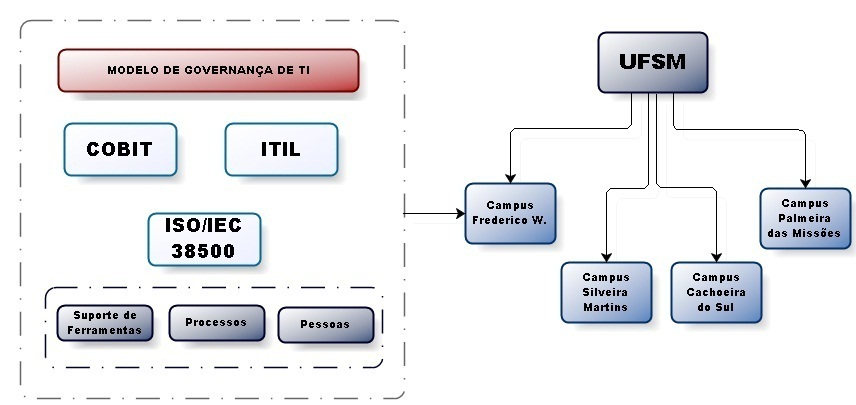
\includegraphics[scale=0.5]{figuras/ModeloGTI.jpg}
\caption{Demonstrativo de estudo de Governan�a de TI em rela��o a UFSM
 campus de Frederico Westphalen }
\label{figura1}  
\end{figure}
 
   \subsubsection{Portf�lio de Servi�os}
   Portf�lio de Servi�os � um conjunto 
   completo de servi�os que ser�o entregues. S�o agrupados por tamanho, 
   disciplina e valor estrat�gico ou seja, o Portf�lio engloba todos os servi�os
   entregues pela organiza��o, ou pela �rea de TI da mesma, tamb�m os que est�o aposentados ou absoleto por de certa forma ainda ser �til para a organiza��o e por �ltimo elemento do portf�lio que n�o podemos esquecer, al�m de servi�os
   ativos e aposentados, s�o os servi�os propostos ou em desenvolvimento. S�o aqueles que 
   ser�o ou n�o servi�os ativos um dia.  A gest�o de portf�lio tem como objetivo gerenciar os servi�os durante todo o ciclo 
   de vida do mesmo. A gest�o do portf�lio � um processo de car�cter estrat�gico e deve 
ser conduzida por uma fun��o que tenha autonomia na organiza��o de TI: cargos de 
diretoria a executivos. Portf�lio de Servi�o � a representa��o
   de todos os servi�os de TI. O gerenciamento do portf�lio serve para organizar investimentos a 
   ser feitos na organiza��o. O Portf�lio de Servi�o est� dividido em tr�s
   partes \cite{ITIL2}:
   \begin{itemize}
   \item O funil de servi�o, ou pipeline de servi�o: que mostra oque est� por
   ser realizado; 
   \item O cat�logo de servi�o: mostra os servi�os que est�o em
    desenvolvimento;
   \item Os servi�os obsoletos: mostra os servi�os que devem ser descartados;
   \end{itemize}
      
 
     Para Filho ~\cite{ITIL} no Portf�lio de Servi�os devem estar posto todos os
     servi�os existentes no Cat�logo de Servi�os da organiza��o. O gerenciamento de servi�os inclui: definir, analisar, aprovar e controla.
     \begin{itemize}
     \item Definir: levantar os dados existentes no Portf�lio, verificando  oque melhorar para agregar valores;
     \item Analisar: analisar as demandas de servi�os para identificar oque agrega valor � organiza��o; 
     \item Aprovar: aprovar o portf�lio proposto autorizando recursos e servi�os futuros;
     \item Controlar: comunicar decis�es, alocar recursos para o inicio de
     atividades, renovar o portf�lio 
    \end{itemize}
  
  A Figura ~\ref{figura 2} apresenta um fluxo de atendimento onde cada chamada tem 
 um in�cio e um fim, onde o usu�rio realiza um chamado atrav�s de email, ou atrav�s 
 do telefone, o t�cnico avalia o chamado e entra em contato com o usu�rio, se o 
 problema puder ser resolvido remotamente o problema estar� resolvido caso n�o seja 
 poss�vel o t�cnico realiza atendimento local, onde resolve o problema, caso n�o 
 consiga mesmo assim ent�o � procurado alternativas poss�vel sendo assim o problema 
 se encerra. A ferramenta Help Desk utilizada pelos t�cnicos do campus de Frederico 
 Westphalen segue enfim esse processo. 
 
  %footnote{Figura etirada do endereço
 %\url{www.getinews.com.br}}
\begin{figure}[H]
\centering
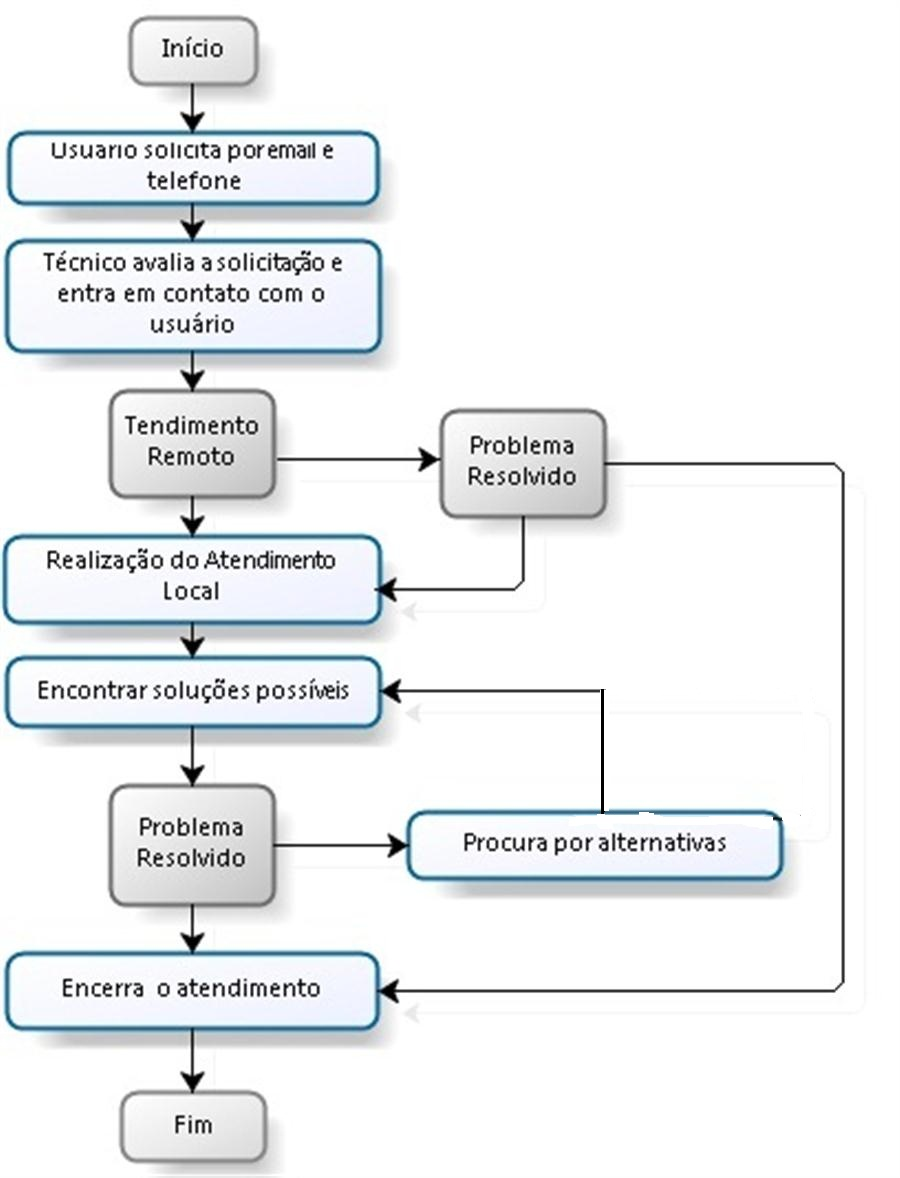
\includegraphics[scale=0.4]{figuras/fluxoAtividade.jpg}
\caption{Fluxo de atividade de atendimento realizados pela equipe de TI} 
\label{figura 2}  
\end{figure}
 
  \subsubsection{Cat�logo de Servi�os} 
  ITIL \cite{ITIL2} define cat�logo de servi�os como "parte do Portf�lio dispon�vel
   para um cliente. S�o os servi�os ativos na vis�o do cliente em espec�fico, este 
   cliente ser� representado por uma organiza��o com a qual mant�m contrato. 
   Na gest�o do cat�logo, o objetivo � que todas as informa��es dos servi�os 
   ativos estejam claramente dispon�veis e especificadas para o clientes. O gestor 
   do processo tem um papel t�tico na presta��o dos servi�os de TI. 

O Cat�logo de Servi�os deve ser entendido como a principal ferramenta de comunica��o 
entre TI e Neg�cio, garantindo que os processos de demanda e oferta de servi�os 
sejam executados de forma eficaz. Um bom Cat�logo de Servi�os � o primeiro passo 
para uma boa Gest�o de Servi�os de TI.
  
  Ainda no ITIL \cite{ITIL2} um Cat�logo de Servi�os, al�m de importante 
  ferramenta de comunica��o e transpar�ncia entre TI e Neg�cio, deve ser 
  entendido como importante ferramenta gerencial na obten��o de informa��es 
  sobre a opera��o. O objetivo do Gerenciamento de Cat�logo de Servi�o � fornecer 
  uma �nica fonte de informa��es consistentes sobre todos os servi�os que est�o acordados para ser entregues aos clientes.
  % por um texto
  
  Ao realizar a analise da pesquisa realizada no setor de TI da universidade
  UFSM no campus de Frederico Westphalen com foco na ferramenta Help Desk
  utilizada pelos t�cnicos de TI, identificando assim, os tipos de servi�os
  prestados pelos membros do setor e quais eram suportados pela ferramenta, 
  dessa forma identificado que a ferramenta atende a apenas um tipo de servi�o 
  sendo ele a Abertura de Chamados, que no momento � usado para controle interno 
  do setor e que essa ferramenta n�o � institucionalizada, ou seja, a 
  popula��o acad�mica n�o faz uso da mesma.

 Nesta ferramenta s�o armazenados dados de diversas formas de atendimentos que s�o solicitados, entre eles instala��o de sistemas operacionais, manuten��o de programas 
instalados para os usu�rios, suporte de redes, em fim necessidades enfrentadas pelos 
usu�rios em rela��o a hardware e software em geral, identificando como cliente toda a 
comunidade acad�mica, professores, t�cnico, alunos e demais funcion�rios da universidade.

  A Tabela ~\ref{suportRedes}, apresenta as informa��es do atendimento 
  realizado na campus de Frederico Westphalen, servi�o este referente a Suporte 
  de Redes, nomeando o servi�o, definindo seu estado, o tipo de servi�o, quem s�o 
  os clientes que s�o beneficiados pelo servi�o, justificando a realiza��o do mesmo, 
  os resultados esperados se existe algum tipo de depend�ncia em rela��o a outros 
  servi�os, se existe algum tipo de mudan�as em projeto para tal servi�o e as
  necessidades de aperfei�oamento dos membros realizadores do servi�o.
 %Figura~\ref{figura 3} Portf�lio de Servi�os %Titulo da figura
  
%\begin{figure}[H]
%\centering
%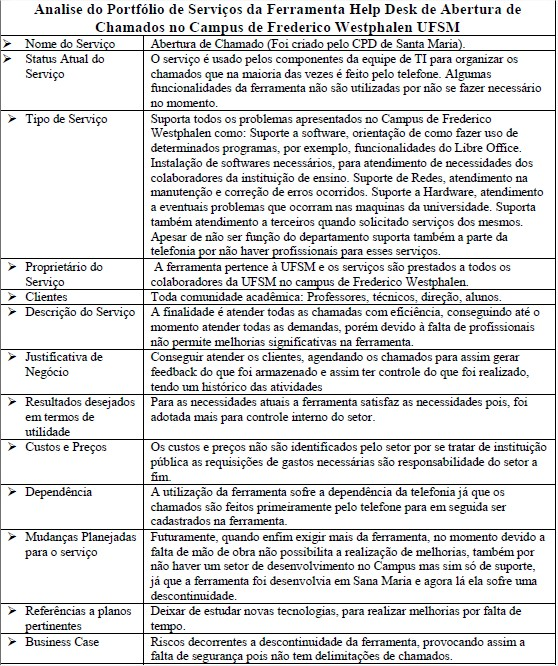
\includegraphics[scale=0.7]{figuras/Portifolio.jpg}
%\caption{Portf�lio de Servi�os da Ferramenta Help Desk de Abertura de Chamados
%no Campus de Frederico Westphalen}
%\label{figura 3}  
%\end{figure}
\begin{table}[H]
\tiny
	\centering
	
	\label{suport}
	\begin{tabular}{|l|l|}
		\hline
		Nome do Servi�o&Suporte de Redes \\
		\hline
		Status Atual do Servi�o&O servi�o � realizado pela equipe de TI da universidade, equipe esta composta de tr�s colaboradores efetivos e dois bolsistas. \\
		\hline
		Tipo de Servi�o&Suporte de Redes, atendimento na manuten��o e corre��o de erros ocorridos,  na rede do campus \\
		\hline
		Clientes&Toda comunidade acad�mica: Professores, t�cnicos, dire��o, alunos. \\
		\hline
		Descri��o do Servi�o&O servi�o � realizado sempre que solicitado, onde � realizado manuten��o de redes j� existentes, onde s�o corrigidos eventuais problemas. \\
		\hline
		Justificativa&Conseguir atender os clientes, para que as dificuldades enfrentadas sejam solucionadas, os dados encontrados geram feedback  \\
		\hline
		Resultados desejados &Satisfa��o do usu�rio, em rela��o a rede, para que assim possam realizar suas atividades   \\
		\hline
		Depend�ncia&O atendimento sofre depend�ncia da telefonia j� que os chamados s�o feitos atrav�s do telefone. \\
		\hline
		Mudan�as Planejadas para o servi�o&A falta de m�o de obra n�o possibilita a realiza��o de melhorias.  \\
		\hline
		Refer�ncias a planos pertinentes&Necessidade de aperfei�oamento, para efetuar melhorias. \\
		\hline
		Business Case&Riscos decorrentes a depend�ncia . \\
		\hline
	\end{tabular}
	%\label{tab:Nome_Da_Tabela}
	\caption{An�lise de Portif�lio: Suporte de Redes}
\end{table} 

A Tabela~\ref{suportSoftf}, est� sendo realizado um atendimento para realizar
suporte a sotwares, sendo relatado o processo da mesma forma que quando atendido
um servi�o de suporte a redes, onde � relatado o nome de servi�os, status do
mesmo, seus clientes, justificativa da realiza��o os resultados desejados e
mudan�as previstas para o servi�o.

\begin{table}[H]
\tiny
	\centering
	\label{suportSoft}
	\begin{tabular}{|l|l|}
		\hline
		Nome do Servi�o&Suporte e instala��o de Software  \\
		\hline
		Status Atual do Servi�o&O servi�o � realizado pela equipe de TI da universidade, equipe esta composta de tr�s colaboradores efetivos e dois bolsistas. \\
		\hline
		Tipo de Servi�o&Suporte a software, orienta��o de  uso de  programas, por exemplo. Instala��o de softwares necess�rios, para atendimento de necessidades. \\
		\hline
		Clientes&Toda comunidade acad�mica: Professores, t�cnicos, dire��o, alunos. \\
		\hline
		Descri��o do Servi�o&Manuten��o de software,  instala��o de softwares, treinamento com usu�rio para utilizar os software requisitado. \\
		\hline
		Justificativa&Conseguir atender os clientes, para que  dificuldades sejam solucionadas, os dados encontrados geram feedback  tendo controle do realizado. \\
		\hline
		Resultados desejados em termos de utilidade&Satisfa��o do usu�rio, em rela��o a os softwares . \\
		\hline
		Depend�ncia&O atendimento sofre depend�ncia da telefonia j� que os chamados s�o feitos atrav�s do telefone. \\
		\hline
		Mudan�as Planejadas para o servi�o&A falta de m�o de obra n�o possibilita a realiza��o de melhorias. \\
		\hline
		Refer�ncias a planos pertinentes&Necessidade de aperfei�oamento, para efetuar melhorias. \\
		\hline
		Business Case&Riscos decorrentes a depend�ncia . \\
		\hline
	\end{tabular}
	\label{tab:Nome_Da_Tabela}
	\caption{An�lise de Portif�lio: Suporte de Softwares}
\end{table} 

A Tabela ~\ref{suportHard} identifica a realiza��o de um atendimento pra
suporte de hardware onde � nomeado o servi�o, identificado seu estatus, quem s�o seus
clientes, descrevendo suas caracteristicas, justificando a realiza��o de tal
atendimento, se ele possui alguma depend�ncia em rela��o a outros servi�os e se
h� previs�o de mudan�as para o servi�o.

\begin{table}[H]
\tiny
\centering
	\label{suportHard}
	\begin{tabular}{|l|l|}
		\hline
		Nome do Servi�o&Suporte a Hardware \\
		\hline
		Status Atual do Servi�o&O servi�o � realizado pela equipe de TI da universidade, equipe esta composta de tr�s colaboradores efetivos e dois bolsistas. \\
		\hline
		Tipo de Servi�o&Suporte a Hardware, atendimento a eventuais problemas que ocorram nas maquinas da universidade. \\
		\hline
		Clientes&Toda comunidade acad�mica: Professores, t�cnicos, dire��o, alunos. \\
		\hline
		Descri��o do Servi�o&O servi�o � realizado sempre que solicitado, onde � realizado manuten��o de hardware, onde s�o corrigidos eventuais problemas. \\
		\hline
		Justificativa&Atender os clientes, para que as dificuldades enfrentadas sejam solucionadas, os dados encontrados geram feedback  tendo controle do que foi realizado. \\
		\hline
		Resultados desejados em termos de utilidade&Satisfa��o do usu�rio, em rela��o a rede, para que assim possam realizar suas atividades  em perfeitas condi��es. \\
		\hline
		Depend�ncia&O atendimento sofre depend�ncia da telefonia j� que os chamados s�o feitos atrav�s do telefone. \\
		\hline
		Mudan�as Planejadas para o servi�o&A falta de m�o de obra n�o possibilita a realiza��o de melhorias.  \\
		\hline
		Refer�ncias a planos pertinentes&Necessidade de aperfei�oamento, para efetuar melhorias. \\
		\hline
		Business Case&Riscos decorrentes a depend�ncia. \\
		\hline
	\end{tabular}
	\label{tab:Nome_Da_Tabela}
	\caption{An�lise de Portif�lio: Suporte de Hardwares}
\end{table}

A Tabela~\ref{terceiro} Est� descrito uma das atividades desenvolvidas pelo 
setor de TI do campus de Frederico Westphalen onde o atendimento a terceiro est� 
relacionado com auxiliar as empresas terceirizadas que iram prestar servi�os na 
universidade prestando informa��es para que o objetivo da a��o seja atingida. 
Dessa norma nomeia o servi�o, estabelece o estado de tal servi�o, quem s�o os 
clientes desse servi�o, justificando a exist�ncia desse servi�o identificando 
qual o resultado esperado, suas depend�ncias.  

\begin{table}[h]
\tiny
	\centering
	\caption{Analise de Portif�lio: Suporte de Terceiros}
		\label{terceiro}
	\begin{tabular}{|l|l|}
		\hline
		Nome do Servi�o&Atendimento a Terceiros \\
		\hline
		Status Atual do Servi�o&O servi�o � realizado pela equipe de TI da universidade, equipe esta composta de tr�s colaboradores efetivos e dois bolsistas. \\
		\hline
		Tipo de Servi�o&Suporte o atendimento a terceiros, em eventuais problemas que ocorram nas atividades terceirizadas da universidade. \\
		\hline
		Clientes&Toda comunidade acad�mica: Professores, t�cnicos, dire��o, alunos. \\
		\hline
		Descri��o do Servi�o&O servi�o � realizado sempre que solicitado, onde � realizado presta��o de informa��es para que seja, corrigidos eventuais problemas. \\
		\hline
		Justificativa&Conseguir atender os clientes, para que dificuldades enfrentadas sejam solucionadas, gerando  feedback  para  \\
		\hline
		Resultados desejados em termos de utilidade&Satisfa��o do usu�rio, em rela��o a rede, para que assim possam realizar suas atividades  em perfeitas condi��es. \\
		\hline
		Depend�ncia&O atendimento sofre depend�ncia da telefonia j� que os chamados s�o feitos atrav�s do telefone. \\
		\hline
		Mudan�as Planejadas para o servi�o&A falta de m�o de obra n�o possibilita a realiza��o de melhorias.  \\
		\hline
		Refer�ncias a planos pertinentes&Necessidade de aperfei�oamento, para efetuar melhorias. \\
		\hline
		Business Case&Riscos decorrentes a depend�ncia. \\
		\hline
	\end{tabular}
	\label{tab:Nome_Da_Tabela}
\end{table}

  


%A Tabela ~\ref{suportRedes} apresenta dados referentes a um per�odo de um ano
% apresentados bimestralmente, organizados em atividades resolvidas at� o prazo,
 %resolu��o do problema, satisfa��o dos usu�rios e atividades realizadas.
 
 
 \subsubsection{Servi�o de Help Desk}
 Segundo Statdlober \cite{J} o servi�o de Help Desk fornece um ponto 
 central de contato entre clientes e funcion�rios para apresentar os incidentes 
 e solicita��es de servi�os, permitindo a organiza��o oferecer um servi�o de alta 
 qualidade a um custo operacional m�nimo. Atrav�s de relat�rios centralizados e da 
 monitora��o de solicita��es automatizadas � poss�vel gerar valor ao neg�cio aumentando 
 consideravelmente a produtividade e reduzindo custos.
 % aqui a Figura desen
 
A Figura~\ref{figura4} apresenta a interface do sistema Help Desk usado pelo 
setor de TI da universidade UFSM campus de Frederico Westphalen, nesta interface 
e solicitado os dados do usu�rio que realizar� a chamada e tamb�m os dados do local
 onde o problema est� instaurado e os dados do equipamento que est� com problema.
  Nos dados de identifica��o � solicitado que o usu�rio coloque seu email, nome e
 matr�cula, para fins de controle, tamb�m nos dados de localiza��o � solicitado uma 
 descri��o do local onde est� instaurado o problema para dessa forma, facilitar o 
 atendimento caso haja a necessidade de deslocamento ao local e tamb�m poder ser 
 identificado posteriormente num feedback os lugares de maior incid�ncia de problemas, 
 posteriormente a descri��o identificada pelo usu�rio do que est� acontecendo com o 
 equipamento, assim o t�cnico possa tomar atitudes para resolver o problema. 
 %Figura~\ref{figura4} Interface Sistema Help Desk%Titulo da figura
  
\begin{figure}[H]
\centering
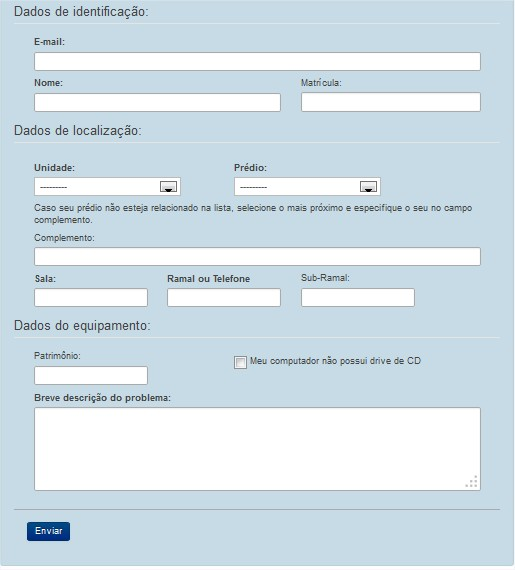
\includegraphics[scale=0.5]{figuras/desen.jpg}
\caption{Interface do Sistema Help Desk usado na UFSM
campus Frederico Westphalen}
\label{figura4}  
\end{figure}

A ferramenta Help Desk n�o � institucionalizada por ser usada somente para
controle interno do setor de TI, dessa forma os dados n�o s�o totalmente atualizados 
e podem n�o conter todas as informa��es existentes.
 
 \subsubsection{Gest�o de Incid�ncias }
 
 No ITIL \cite{ITIL2} o Gerenciamento de Incidentes tem como foco principal reestabelecer servi�o, minimizando o impacto negativo no neg�cio, uma solu��o de contorno ou reparo r�pido fazendo com que o cliente volte a trabalhar. Garantir que os melhores n�veis de disponibilidade e de qualidade dos servi�os, mantendo os acordos de n�vel de servi�o � tamb�m uma tarefa da ger�ncia de incidentes.
 % Aqui a figura Tabela1.pdf
 
 A Figura~\ref{figura5} apresenta as  atividades do Sistema de Chamadas com as
 atividades  realizadas pelo setor de TI da universidade e cadastradas no Sistema, 
 dados este coletados no decorrer de um ano, onde est�o organizados bimestralmente, 
 ou seja os relat�rios s�o apresentados de dois em dois meses, descritos em n�meros  
 decimais e acompanhados do porcentual que cada atividade representa em um �mbito geral.

Ao analisar a figura � poss�vel detectar que o principal motivo para abertura de
chamadas � relacionadas as impressoras da universidade, em seguida est�o problemas
relacionados � rede da universidade, tamb�m � poss�vel observar que existem servi�os que nunca tiveram 
solicita��o de chamados. Tamb�m � poss�vel observar que, nos anos de janeiro e
fevereiro, correspondente aos meses de f�rias letivas as chamadas s�o menores,
devido a menor utiliza��o de equipamentos 
 
 %Figura~\ref{figura5} Sistema de Chamadas dos meses  %Titulo da figura 
%  % Please add the following required packages to your document preamble:
% \usepackage[normalem]{ulem}
% \useunder{\uline}{\ul}{}
\begin{table}[h]
\tiny

\centering
\caption{Sistema de Chamada dos Meses}
\label{sistChamada}
\begin{tabular}{|l|l|l|l|l|l|l|l|l|l|l|l|l|}
\hline
\multicolumn{13}{|c|}{Sistema de Chamada dos meses}                                                                                                                                                                                                                                            \\ \hline
\multicolumn{13}{|l|}{}                                                                                                                                                                                                                                                                        \\ \hline
M�s/Ano                                                              & \multicolumn{2}{l|}{Maio/Jun 2014} & \multicolumn{2}{l|}{Jul /Ago 2014} & \multicolumn{2}{l|}{Set/Out 2014} & \multicolumn{2}{l|}{Nov/Dez 2014} & \multicolumn{2}{l|}{Jan/Fev 2015} & \multicolumn{2}{l|}{Mar/Abr 2015} \\ \hline
\multicolumn{13}{|l|}{}                                                                                                                                                                                                                                                                        \\ \hline
Atividades Atuais                                                    & NUM           & \%                 & NUM           & \%                 & NUM           & \%                & NUM           & \%                & NUM           & \%                & NUM           & \%                \\ \hline
Instala��o/ problemas desw b�sicos (SO,Navegador, Antiv�rus)         & 6             & 17,14\%            & 6             & 13,33\%            & 2             & 11,11\%           & 1             & 5,56\%            & 3             & 60,00\%           & 1             & 7,69\%            \\ \hline
Drivers/Codecs                                                       & 2             & 5,71\%             & 2             & 44,44\%            & 0             & 0,00\%            & 0             & 0,00\%            & 1             & 20,00\%           & 0             & 0,00\%            \\ \hline
SIE                                                                  & 2             & 5,71\%             & 5             & 11,11\%            & 1             & 5,56\%            & 1             & 5,56\%            & 1             & 20,00\%           & 2             & 15,38\%           \\ \hline
Ponto de rede                                                        & 1             & 2,86\%             & 1             & 2,22\%             & 0             & 0,00\%            & 0             & 0,00\%            & 0             & 0,00\%            & 0             & 0,00\%            \\ \hline
Impressora                                                           & 5             & 14,29\%            & 5             & 11,11              & 2             & 11,11\%           & 7             & 38,89\%           & 0             & 0,00\%            & 5             & 38,46             \\ \hline
Formata��o                                                           & 3             & 8,57\%             & 0             & 0,00\%             & 0             & 0,00\%            & 0             & 0,00\%            & 0             & 0,00\%            & 0             & 0,00\%            \\ \hline
Ativa��o do proxy                                                    & 0             & 0,00\%             & 0             & 0,00\%             & 1             & 5,56\%            & 0             & 0,00\%            & 0             & 0,00\%            & 0             & 0,00\%            \\ \hline
Troca de Perif�rico                                                  & 2             & 5,71\%             & 2             & 4,44\%             & 2             & 11,11\%           & 2             & 11,11\%           & 0             & 0,00\%            & 0             & 0,00\%            \\ \hline
Instala��o/remo��o de softwares espec�ficos (statistic, sigepweb,..) & 0             & 0,00\%             & 1             & 2,22\%             & 3             & 16,67\%           & 0             & 0,00\%            & 0             & 0,00\%            & 0             & 0,00\%            \\ \hline
Cadastrar MAC                                                        & 0             & 0,00\%             & 0             & 0,00\%             & 0             & 0,00\%            & 0             & 0,00\%            & 0             & 0,00\%            & 0             & 0,00\%            \\ \hline
Softwares de escrit�rio(Office, Leitor de PDF)                       & 0             & 0,00\%             & 3             & 6,67\%             & 1             & 5,56\%            & 4             & 22,22\%           & 0             & 0,00\%            & 0             & 0,00\%            \\ \hline
Sistemas do governo(SIAFI, SCDP, Token)                              & 0             & 0,00\%             & 0             & 0,00\%             & 0             & 0,00\%            & 0             & 0,00\%            & 0             & 0,00\%            & 0             & 0,00\%            \\ \hline
Remo��o v�rus/ Spyware                                               & 2             & 5,71\%             & 2             & 4.44\%             & 2             & 11,11\%           & 1             & 5,56\%            & 0             & 0,00\%            & 1             & 7,69\%            \\ \hline
Instala��o decomputadores                                            & 4             & 11,43\%            & 4             & 8,89               & 0             & 0,00\%            & 0             & 0,00\%            & 0             & 0,00\%            & 1             & 7,69              \\ \hline
Instala��o/troca oumanuten��o de roteador                            & 0             & 0,00\%             & 0             & 0,00\%             & 0             & 0,00\%            & 0             & 0,00\%            & 0             & 0,00\%            & 0             & 0,00\%            \\ \hline
Rede                                                                 & 5             & 14,29\%            & 6             & 13,33\%            & 1             & 5,56\%            & 0             & 0,00\%            & 0             & 0,00\%            & 1             & 7,69\%            \\ \hline
Ponto Eletr�nico                                                     & 0             & 0,00\%             & 0             & 0,00\%             & 0             & 0,00\%            & 0             & 0,00\%            & 0             & 0,00\%            & 0             & 0,00\%            \\ \hline
Conflito de IP                                                       & 0             & 0,00\%             & 0             & 0,00\%             & 0             & 0,00\%            & 0             & 0,00\%            & 0             & 0,00\%            & 0             & 0,00\%            \\ \hline
Datashow / Projetores                                                & 0             & 0,00\%             & 2             & 4,44\%             & 0             & 0,00\%            & 0             & 0,00\%            & 0             & 0,00\%            & 0             & 0,00\%            \\ \hline
Configura��o de e-mail                                               & 0             & 0,00\%             & 0             & 0,00\%             & 0             & 0,00\%            & 0             & 0,00\%            & 0             & 0,00\%            & 0             & 0,00\%            \\ \hline
Outros                                                               & 3             & 8,57\%             & 6             & 13,33\%            & 3             & 16,67\%           & 2             & 11,11\%           & 0             & 0,00\%            & 2             & 15,38\%           \\ \hline
Total                                                                & 35            & 100,00\%           & 45            & 100,00\%           & 18            & 100,00\%          & 18            & 100,00\%          & 5             & 100,00\%          & 13            & 100,00\%          \\ \hline
\end{tabular}
\end{table}
  
 
\begin{figure}[H]
\centering
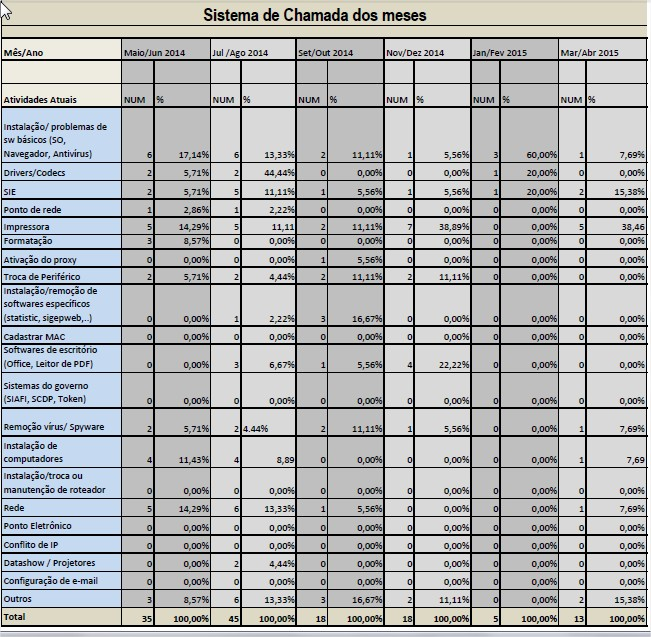
\includegraphics[scale=0.7]{figuras/tabela1.jpg}
\caption{A figura demonstra as atividades realizadas no periodo de um ano}
\label{figura5}  
\end{figure}



 % aqui a figura Tabela
 
 %Figura~\ref{figura6} Indicadores do Sistema de Chamadas %Titulo da figura
  
%\begin{figure}[H]
%\centering
%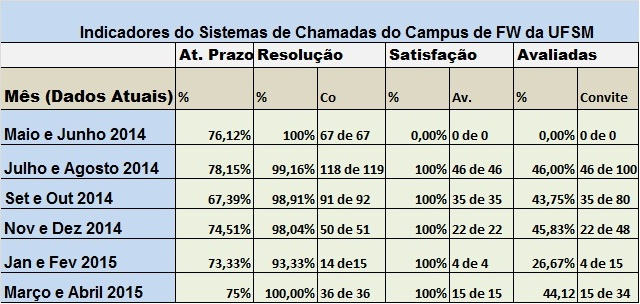
\includegraphics[scale=0.5]{figuras/Tabela.jpg}
%\caption {Demonstrativo do Sistema de Chamadas}
%\label{figura6}  
%\end{figure}
\begin{table}[h]
\centering
\caption{My caption}
\label{my-label}
\begin{tabular}{|l|l|l|l|l|l|l|l|}
\hline
\multicolumn{8}{|l|}{Indicadores do Sistemas de Chamadas do Campus de FW da UFSM}                                                                        \\ \hline
                    & \multicolumn{1}{c|}{At. Prazo} & \multicolumn{2}{c|}{Resolu��o} & \multicolumn{2}{c|}{Satisfa��o} & \multicolumn{2}{c|}{Avaliadas} \\ \hline
M�s (Dados Atuais)  & \%                             & \%            & Co             & \%            & Av.             & \%            & Convite        \\ \hline
Maio e Junho 2014   & 76,12\%                        & 100\%         & 67 de 67       & 0,00\%        & 0 de 0          & 0,00\%        & 0 de 0         \\ \hline
Julho e Agosto 2014 & 78,15\%                        & 99,16\%       & 118 de 119     & 100\%         & 46 de 46        & 46,00\%       & 46 de 100      \\ \hline
Set e Out 2014      & 67,39\%                        & 98,91\%       & 91 de 92       & 100\%         & 35 de 35        & 43,75\%       & 35 de 80       \\ \hline
Nov e Dez 2014      & 74,51\%                        & 98,04\%       & 50 de 51       & 100\%         & 22 de 22        & 45,83\%       & 22 de 48       \\ \hline
Jan e Fev 2015      & 73,33\%                        & 93,33\%       & 14 de15        & 100\%         & 4 de 4          & 26,67\%       & 4 de 15        \\ \hline
Mar�o e Abril 2015  & 75\%                           & 100,00\%      & 36 de 36       & 100\%         & 15 de 15        & 44,12         & 15 de 34       \\ \hline
\end{tabular}
\end{table}


A Tabela ~\ref{indicador} apresenta dados referentes a um per�odo de um ano apresentados bimestralmente, organizados em atividades resolvidas at� o prazo, resolu��o do problema, satisfa��o dos usu�rios e atividades realizadas. 
 
 Nas atividades realizadas at� o prazo o percentual est� sendo colocado desconsiderando 
 que as atividades s�o armazenadas em um prazo de 48 horas corridos n�o considerando assim 
 s�bados e domingos, nem feriados dessa forma o percentual n�o � preciso. 

� poss�vel observar que a resolu��o dos problemas ocorridos � muito satisfat�ria j� que em quase todos os meses e quase atingido totalmente.  A satisfa��o em rela��o aos atendimentos � total em todos os meses, e o percentual de pessoas que avaliam os atendimentos s�o vari�veis, j� que o �ndice de avalia��o e baixo em propor��o a quantidade de solicita��es de atendimento. Tamb�m � poss�vel observar que em meses que correspondem a f�rias escolares o atendimento � reduzido consideravelmente, devido a um menor uso de hardware e software no campus.

  %\begin{table}[h]
\centering
\caption{My caption}
\label{my-label}
\begin{tabular}{|l|l|l|l|l|l|l|l|}
\hline
\multicolumn{8}{|l|}{Indicadores do Sistemas de Chamadas do Campus de FW da UFSM}                                                                        \\ \hline
                    & \multicolumn{1}{c|}{At. Prazo} & \multicolumn{2}{c|}{Resolu��o} & \multicolumn{2}{c|}{Satisfa��o} & \multicolumn{2}{c|}{Avaliadas} \\ \hline
M�s (Dados Atuais)  & \%                             & \%            & Co             & \%            & Av.             & \%            & Convite        \\ \hline
Maio e Junho 2014   & 76,12\%                        & 100\%         & 67 de 67       & 0,00\%        & 0 de 0          & 0,00\%        & 0 de 0         \\ \hline
Julho e Agosto 2014 & 78,15\%                        & 99,16\%       & 118 de 119     & 100\%         & 46 de 46        & 46,00\%       & 46 de 100      \\ \hline
Set e Out 2014      & 67,39\%                        & 98,91\%       & 91 de 92       & 100\%         & 35 de 35        & 43,75\%       & 35 de 80       \\ \hline
Nov e Dez 2014      & 74,51\%                        & 98,04\%       & 50 de 51       & 100\%         & 22 de 22        & 45,83\%       & 22 de 48       \\ \hline
Jan e Fev 2015      & 73,33\%                        & 93,33\%       & 14 de15        & 100\%         & 4 de 4          & 26,67\%       & 4 de 15        \\ \hline
Mar�o e Abril 2015  & 75\%                           & 100,00\%      & 36 de 36       & 100\%         & 15 de 15        & 44,12         & 15 de 34       \\ \hline
\end{tabular}
\end{table}
  
%\ldots
 
  \section{Roteiro de Implanta��o}
\label{sec:roteiroDeImplantacao} 
 
 Planejamento � a palavra chave para as organiza��es, pois atrav�s dele h� a possibilidade de 
 abrang�ncias competitivas, quando n�o existe planejamento estrat�gico n�o h� conscientiza��o 
 da dire��o em rela��o ao plano estrat�gico de TI e sua necessidade para sustentar metas de 
 neg�cio. O planejamento possibilita a aquisi��o de maturidade \cite{Cobit}.

Para que seja poss�vel acontecer a Governan�a de TI � necess�ria uma sensibiliza��o de 
todas as partes envolvida na organiza��o, mas principalmente da dire��o, pois � atrav�s 
dela que eventuais problemas poder�o ser solucionados ou amenizados, \cite{f}.
 
 Com base no modelo proposto por \cite{f} torna se poss�vel desenvolver um
 roteiro  � ser proposto para desenvolver na UFSM campus de Frederico
 Westphalen onde foi selecionado cinco passos de implanta��o e.
 
  \subsection{Mapeamento de Servi�os usando ITIL} 
 
   A ITIL~\cite{ITIL2} diz que o mapeamento de servi�o � estabelecer como o
servi�o vai proceder, como vai ser controlado e desenhado. Para isso � necess�rio 
uma esquematiza��o, utilizando Portf�lio de Servi�os e Catalogo de Servi�os.
 
   A Figura ~\ref{figura1} representa um modelo de Governan�a de TI, com seus
principais frameworks de governan�a, COBIT, ITIL e ISO/IEC38500. A figura
 ~\ref{figura1} apresenta um esbo�o da  UFSM que
al�m do campus principal em Santa Maria ainda possui 4 campus distribu�dos no interior do 
 estado, dessa forma a figura demonstra que o estudo est� sendo realizado em um desses 
 campus do interior do estado, mais especificadamente o campus de Frederico Westphalen, 
 este estudo buscando identificar ferramentas j� utilizadas, poss�veis ferramentas que 
 poder�o ser suportadas pela mesma.
  
\begin{figure}[H]
\centering
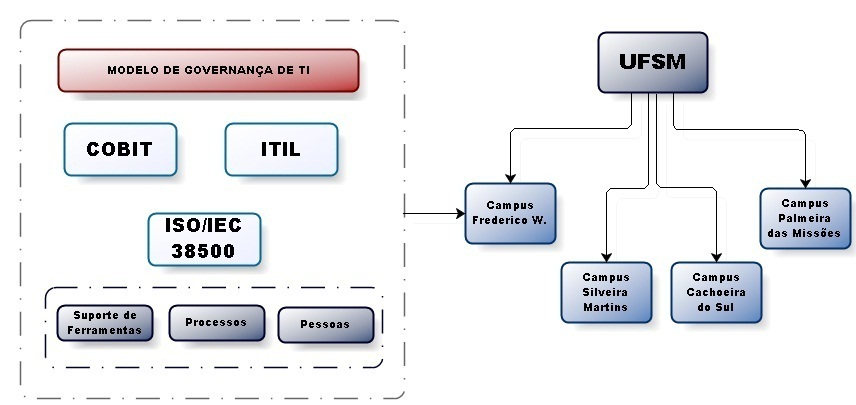
\includegraphics[scale=0.5]{figuras/ModeloGTI.jpg}
\caption{Demonstrativo de estudo de Governan�a de TI em rela��o a UFSM
 campus de Frederico Westphalen }
\label{figura1}  
\end{figure} 
 
 A Figura~\ref{f19} apresentado um poss�vel plano de implanta��o de
Governan�a de TI no Campus de Frederico Westphalen delimitando ac�es que
direcionariam a implanta��o da mesma, dessa forma seriam oito passo que
trilhariam as a��es at� chegar a aprova��o do programa, em en sequencia a
elabora��o de planos de gerencia de mudan�as e aprimoramento da implanta��o,
implantando os projetos, monitorando os mesmos, avaliando para dessa forma
comunicar os resultados.
 %\begin{itemize}
\begin{figure}[H] 
\centering
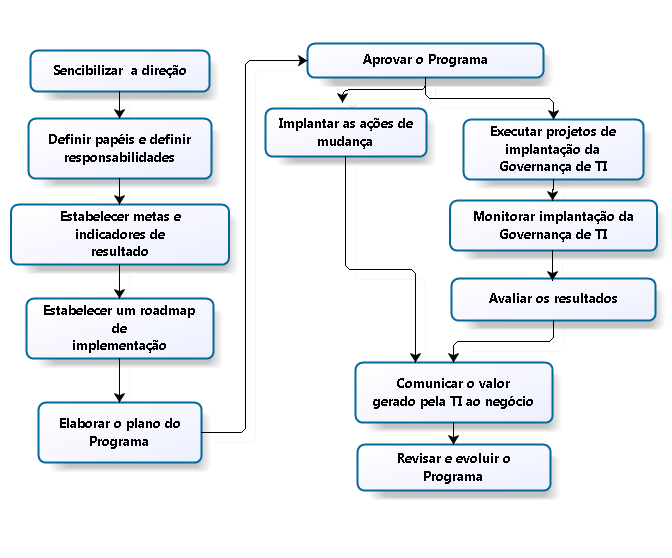
\includegraphics[scale=0.6]{figuras/rotImpl.png}
\caption{Projeto de Roteiro de Implanta��o no Campus de FW }
\label{f19}  
\end{figure}

\begin{itemize}
\item Sensibilizar a dire��o: ter o apoio da dire��o para dessa forma conseguir
angariar recursos para desenvolve as atividades necess�rias na implanta��o de Governan�a 
de TI. Para fundamentar essa a��o pode ser usado de
v�rios instrumentos entre eles palestras, visitas a outras organiza��es que j� fazem
uso de Governan�a de TI, mostrando poss�veis resultados que a mesma pode gerar;
\item Definir pap�is e definir responsabilidades: definir quem realizara cada. 
	atividade e a responsabilidade que ter� em rela��o a tal atividade para dessa 
	forma atingir ao objetivo final, (alta administra��o, �rea de auditoria,
compliance e riscos, desenvolvimento, suporte, infraestrutura tecnol�gica, seguran�a
da informa��o);
\item Estabelecer metas e indicador final: Tra�aras a��es, determinar oque se quer
ter ao final dessas a��es e de que forma se pretende chegar ao final dessas a��es; 

\item Estabelecer um roadmap de implanta��o: estabelecendo a��es de curto m�dio
e longo prazo, identificando as a��es de maior prioridade. Identificar o que
precisa ser feito, definir a sequencia das atividades a ser implantadas, 
identificando os benef�cios que poder�o ser alcan�ados;
\item Elaborar o plano do programa: definir quais projetos faram parte do
programa, definir escopo. Ap�s ter o roadmap delimitar
quais projetos que faram parte do programa, delimitando escopo, estrutura
e a��es de TI, sequencia de implanta��o dos processos, em um linha de tempo pr�
estabelecida.
\item Aprovar o programa: Ap�s ter o plano pronto realizar a aprova��o do mesmo
para dar in�cio a implanta��o de Governan�a de TI; 
\item Implantar as a��es de mudan�a: por em pr�tica oque foi planejado;
\item Executar os projetos de implanta��o de Governan�a de TI: Executar oque
anteriormente foi planejado de forma organizada; 
\item Monitorar a implanta��o: Realizar o monitoramento para prever necessidades
d mudan�as ou realizar altera��es no plano;
\item Avaliar os resultados: Avaliar para definir os pr�ximos passos;
\item Comunicar os resultados alcan�ados: Tomar decis�es em conjunto � a melhor
 forma de se ter sucesso; 
 \item	Revisar e evoluir o programa: Adaptar o plano para dessa forma ter
 sucesso nos passos futuros.
\end{itemize}
%\end{referencialTeorico}

  \section{CITSMART}
\label{sec:citsmart}

 O Citsmart � um software de gest�o de TI, que implementa conceitos e
 tecnicas de Governan�a de TI.  Citsmart tem como objetivo manter a efici�ncia
 nos processos de presta��o de servi�os e promover sua melhoria \cite{Citsmart}.
 
A Figura~\ref{f15} demonstra a cria��o de servi�os no
software CITSMART esta figura est� demonstrada a cria��o de um servi�o de 
suporte de redes realizado na UFSM campus de FW servi�o este 
que est� sendo listado nas tabelas da se��o 5.4 , onde  foi obtido dados pela
pesquisa utilisando cat�logo de servi�os do ITIL dos sevi�os realizados pelo
setor de TI, demonstrando a possibilidade de utiliza��o desta ferramenta para
controle destes dados .

  \begin{figure}[H]
\centering
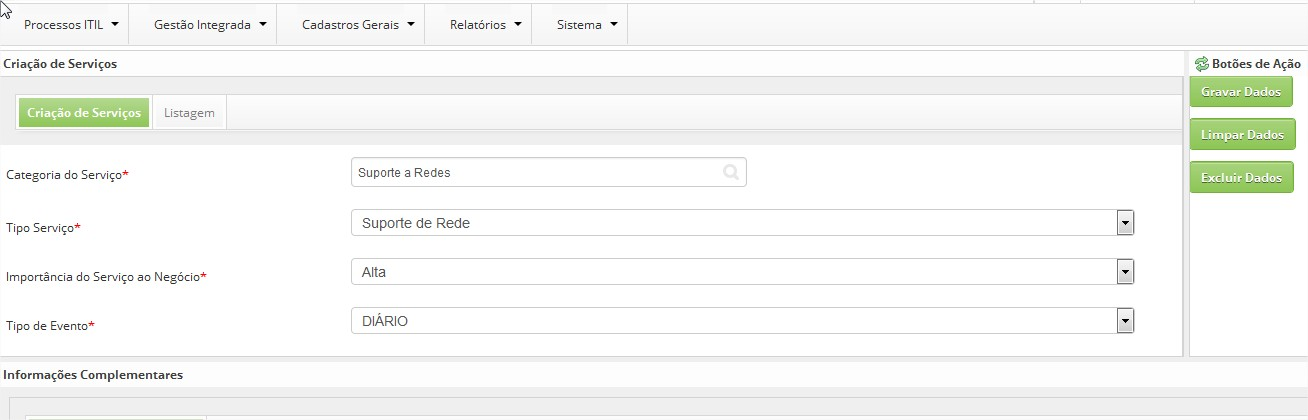
\includegraphics[scale=0.3]{figuras/cadastroRede.jpg}
\caption{Interface demonstrando o cadastro de servi�os  de Redes
CITSMART }
\label{f15}  
\end{figure} 

  A Figura~\ref{figura16} representa um exemplo ficticio de listagem de servi�os
  realizados e previmente cadastrados na ferramenta CITSMART. Dessa forma
  possibilitando uma melhor navega��o e visualiza��o da ferramenta.
  
\begin{figure}[H]
\centering
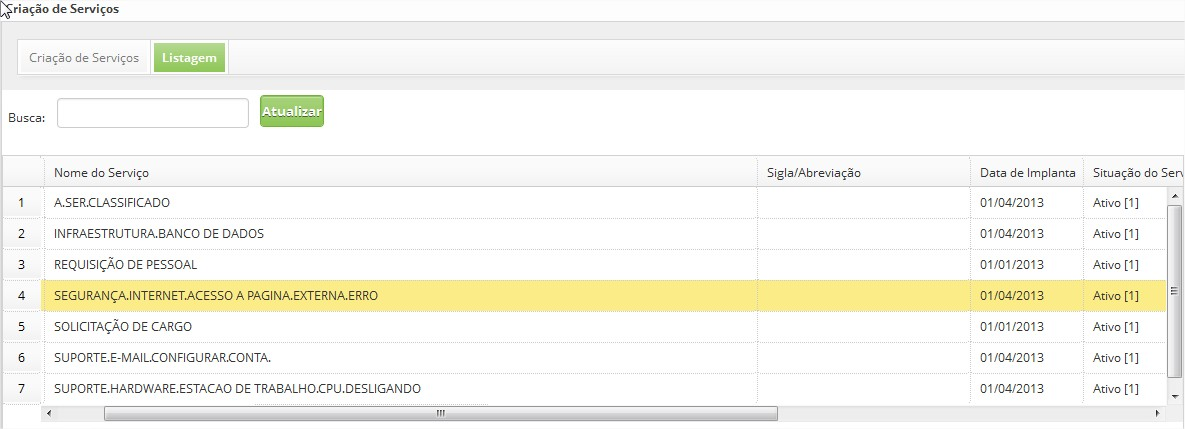
\includegraphics[scale=0.3]{figuras/listaServicos.jpg}
\caption{Interface de cadastro de servi�os  de Software CITSMART}
\label{figura16}  
\end{figure}
 A Figura ~\ref{figura8}  est� representada uma interface  do gerenciador de
cadastro de solicita��es e chamado de atendimento do sistema CITSMART, nessa interface 
est�o organizados os chamados com a numera��o do chamado o tipo de servi�o que foi solicitado, 
tamb�m se � incidente ou requisi��o e a data de cria��o de tal chamado, a prioridade do 
chamado e o prazo limite para a execu��o do chamado e tamb�m o estado que ele se encontra 
se em execu��o, encerado ou em prazo normal de execu��o. 

 \begin{figure}[H]
\centering
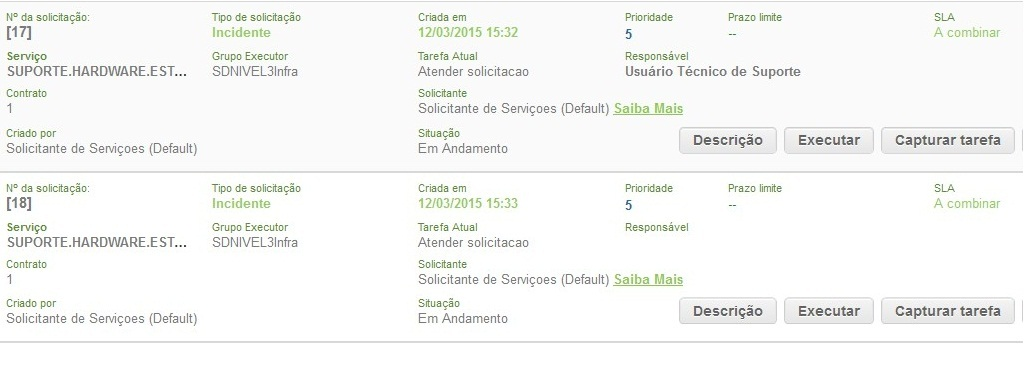
\includegraphics[scale=0.5]{figuras/solicitacao.jpg}
\caption{Interface de Gerenciador de Cadastro de Solicita��es }
\label{figura8}  
\end{figure}

A Figura ~\ref{figura9} apresenta um exemplo de relat�rios do sistema
CITSMART. Neste exemplo esta sendo posto os prazos de atendimento das atividades
cadastradas na ferramenta CITSMART, podendo estar eles em prazo normal, vencidos ou prazo 
a vencer, relacionando a quantidade de cada atividade a seu prazo. Tamb�m � colocada a 
prioridade de cada atividade que pode ser de 1 a 5 dependendo de sua import�ncia e dessa 
forma determinar qual devera ser realizado primeiro. Outra forma de relat�rio � gerada em 
gr�fico para uma melhor visualiza��o destas informa��es.
 \begin{figure}[H]
\centering
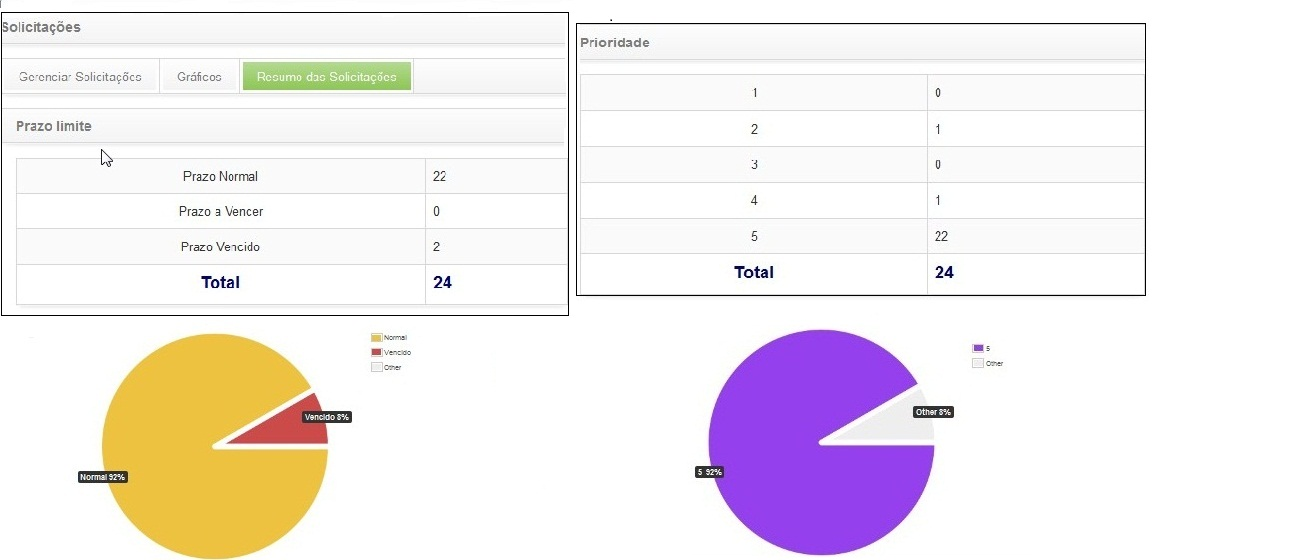
\includegraphics[scale=0.4]{figuras/solicitaPrio.jpg}
\caption{Interface de tipos de relat�rios gerados  pelo
software CITSMART}
\label{figura9}  
\end{figure}


 
  \section{An�lise do Question�rio Aplicado}
\label{sec:analise}

Nesta se��o s�o apresentados os resultados obtidos por meio da aplica��o de um
instrumento, que teve como objetivo colher informa��es e opini�es da pessoas que 
est�o envolvidas no cotidiano da UFSM campus de Frederico Westphalen  visando 
identificar a vis�o dos entrevistados sobre a infraestrutura tecnol�gica do mesmo, 
o conhecimento que tem sobre a import�ncia de se ter a equipe de TI em perfeitas 
condi��es de trabalho e o grau de satisfa��o que a comunidade acad�mica apresenta 
em rela��o a equipe e equipamentos dispon�veis no campus. O instrumento utilizado 
foi baseado no plano diretor de tecnologia da informa��o.

O instrumento proposto foi subdividido entre os temas Sistema de Informa��o, Servi�os 
Dispon�veis, Infraestrutura, Equipe de TI, Conhecimento que a comunidade acad�mica tem 
em rela��o a tais contextos, tamb�m o grau de satisfa��o da mesma em rela��o a estes 
processos. O mesmo foi aplicado em outubro do ano de 2015, pelo autor deste artigo, atrav�s 
do envio de um question�rio montado na ferramenta Google Forms, para toda a comunidade 
acad�mica, professores, t�cnicos, alunos. 

Num primeiro momento foi realizado um pergunta extra pesquisa do conte�do de
Governan�a de TI para saber se quem estava respondendo o question�rio tinha que papel 
na universidade. Em rela��o a esta pergunta onde foram obtido 59 respostas sendo
dessas 21 de alunos (35,6\%), 15 t�cnicos (25,4\%) e 23 professores (39\%), mostrando que
abrangeu todas as �reas da universidade.

A primeira quest�o. \textit{'' Em se tratando de Sistemas de Informa��o. Os
recursos de tecnologia de informa��o dispon�veis s�o suficientes para atender os objetivos da UFSM campus 
Frederico Westphalen''}. Foi dividido em t�picos.
\begin{itemize}
\item \textit{''Portais SIE-Web''} (Portal do Professor, do RH, Produ��o
Institucional, Portal do Aluno, etc.), obteve 59 respostas onde 4 pessoas responderam concordar 
totalmente com a quest�o (6,8\%), 42 concordaram (71,2\%), 2 manifestaram se
indiferentes (3,4\%) e 11 discordaram (18,6\%).
\item \textit{''P�gina Web da UFSM''}, obteve 59 respostas onde 9 pessoas
responderam concordar totalmente com a quest�o (15,3\%), 28 concordaram
(47,5\%), 8 manifestaram se indiferentes (13,6\%) e 14 discordaram (23,7\%).
\item \textit{'' Ferramentas de comunica��o (p�ginas web, blogs, not�cias, redes
sociais, etc.)''}, obteve 59 respostas onde 8 pessoas responderam concordar
totalmente com a quest�o (13,6\%), 31 concordaram (52,5\%), 8 manifestaram se indiferentes (13,6\%), 10
  discordaram (16,9\%) e 2 discordam totalmente (3,4\%).
\item \textit{'' Ferramentas de apoio � educa��o (apres. de slides, v�deos,
elabora��o de texto, etc.)''}, obteve 59 respostas onde 7 pessoas responderam
concordar totalmente com a quest�o (12,1\%), 26 concordaram (44,8\%), 10 manifestaram se
 indiferentes (17,2\%), 12 discordaram (20,7\%) e 3 discordam totalmente
 (5,2\%).
\item \textit{'' Moodle''}, obteve 59 respostas onde 10 pessoas responderam
concordar totalmente com a quest�o (16,9\%), 21 concordaram (35,6\%), 19 manifestaram
 se indiferentes (32,2\%), 7 discordaram (11,9\%) e 2 discordam
 totalmente(3,4\%).
\item \textit{''Outros aplicativos e/ou planilhas para controle interno''},
obteve 59 respostas onde 1 pessoas responderam concordar totalmente com a
quest�o (1,7\%), 17 concordaram (28,8\%), 30 manifestaram se indiferentes
(50,8\%), 10 discordaram (16,9\%) e 1 discordam totalmente (1,7\%). Neste mesmo
t�pica foram dadas varias sugest�es de poss�veis melhorias entre elas algum aplicativo
 que auxilie a fazer agendamentos no RU e um sistema para inscri��o em eventos 
 (que pudesse ser parametrizado para atender diferentes eventos da UFSM), al�m de um 
 sistema que permitisse realizar uma das partes da avalia��o institucional, que � a 
 avalia��o interna de cada curso junto aos discentes.
 \end{itemize}
   
\begin{figure}[H]
\centering
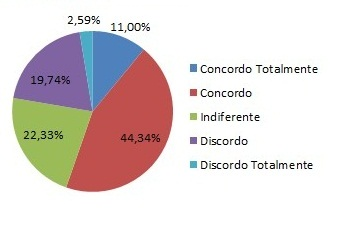
\includegraphics[scale=0.7]{figuras/questao11.jpg}
\caption{Gr�fico relacionado a quest�o 1 do question�rio de Governan�a de TI }
\label{figura10}  
\end{figure}
A Figura ~\ref{figura10} est� resumindo os dados relacionados a sistemas de
informa��o de TI na UFSM campus de Frederico Westphalen.
 
A segunda quest�o. \textit{''EM SE TRATANDO DE SERVI�OS. Os recursos de
Tecnologia de Informa��o dispon�veis s�o suficientes para atender os objetivos da UFSM
campus Frederico Westphalen''}.
 Foi dividido em t�picos.
 \begin{itemize}
\item \textit{''Suporte''}, obteve 59 respostas onde 8 pessoas responderam
concordar totalmente com a quest�o (13,6\%), 34 concordaram (57,6\%), 8
manifestaram se  indiferentes (13,6\%), 7 discordaram (11,9\%) e 2 discordam
totalmente (3,4\%).
\item \textit{''Capacita��o''}, obteve 59 respostas onde 6 pessoas responderam
concordar totalmente com a quest�o (10,2\%), 26 concordaram (44,1\%), 12 manifestaram se
indiferentes (20,3\%), 14 discordaram (23,7\%) e 1 discordam totalmente (1,7\%).
\item \textit{'' D�vidas, orienta��es, etc.''}, obteve 58 respostas onde 7
pessoas responderam concordar totalmente com a quest�o (12,1\%), 31 concordaram
(53,4\%), 9 manifestaram se indiferentes (15,5\%) e 11 discordaram (19\%).
Esta quest�o levanta a necessidade de melhorias, para assim poder se atingir de 
uma forma mais ampla todo o setor requente de servi�os.
\end{itemize}

\begin{figure}[H]
\centering
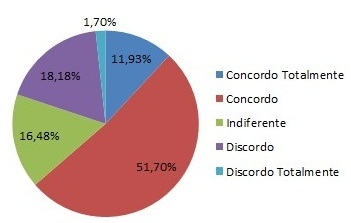
\includegraphics[scale=0.7]{figuras/questao22.jpg}
\caption{Gr�fico relacionado a quest�o 1 do question�rio de Governan�a de TI }
\label{figura11}  
\end{figure}
A Figura ~\ref{figura11} est� resumindo os dados relacionados a servi�os
de TI na UFSM campus de Frederico Westphalen.

A terceira quest�o.\textit{ ''EM SE TRATANDO DE INFRAESTRUTURA. Os recursos de
Tecnologia de Informa��o dispon�veis s�o suficientes para atender os objetivos da UFSM campus Frederico
 Westphalen''}. Foi dividido em t�picos.
 
 \begin{itemize}
\item \textit{''Equipamentos''}, obteve 59 respostas onde 2 pessoasresponderam
concordar totalmente com a quest�o (3,4\%), 21 concordaram (35,4\%), 2 manifestaram se indiferentes
(3,4\%), 27 discordaram (45,8\%) e 7 discordam totalmente (11,9\%).
\item \textit{''Redes''}, obteve 59 respostas onde 12 concordaram (20,3\%),
12 manifestaram se indiferentes (20,3\%), 25 discordaram (42,4\%) e 10 discordam
totalmente (16,9\%).
\item\textit{'' Internet''}, obteve 59 respostas onde 10 concordaram
(16,9\%), 5 manifestaram se indiferentes (8,5\%), 26 discordaram (44,1\%) e 18
discordam totalmente (30,5\%).
Essa quest�o mostra que a comunidade acad�mica est� � espera de melhorias, 
ou seja, h� a necessidade de investimento na melhoria tanto de redes, internet e 
equipamentos.
\end{itemize}

\begin{figure}[H]
\centering
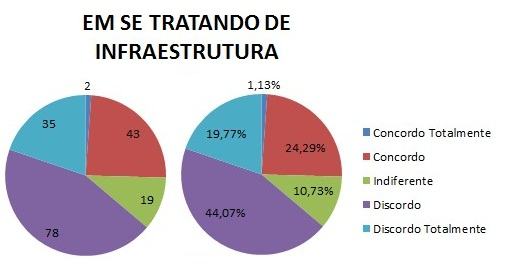
\includegraphics[scale=0.7]{figuras/questao33.jpg}
\caption{Gr�fico relacionado a quest�o 1 do question�rio de Governan�a de TI }
\label{figura12}  
\end{figure}
A Figura ~\ref{figura12} est� resumindo os dados relacionados a infraestrutura
de TI na UFSM campus de Frederico Westphalen.

Na quest�o.\textit{'' Quanto � equipe de Tecnologia de Informa��o, Comentar
sobre a import�ncia:''}
foi  abordada a atua��o  da equipe e sua import�ncia para a UFSM campos de Frederico 
Westphalen, onde foi obtido como resposta. A equipe � de fundamental import�ncia, pois 
sem eles n�o tem como a Universidade caminhar, por exemplo, quando da problema na 
internet eles que tentam resolver ou entram em contato para resolverem, qualquer 
problema nos equipamentos s�o eles que s�o chamados, ou seja a universidade n�o anda 
sem essa equipe. A equipe do N�cleo de Inform�tica auxilia em muito nas atividades 
desempenhadas pelo nosso Departamento (DTecInf) e Curso (Sistemas de Informa��o), 
ajudando a manter os laborat�rios de inform�tica em funcionamento (hardware e software), 
al�m do apoio aos eventos, tais como a JASI (Jornada Acad�mica de Sistemas de Informa��o)
e o Encontro do GDG MAU (Grupo de Desenvolvedores Google do M�dio Alto Uruguai), entre 
outros.

Na quest�o.\textit{'' Coment�rios e sugest�es sobre o assunto: onde foi obtida
resposta como''}:
Melhorias nos sistemas de internet, telefonia, treinamentos para que professores de 
distintas �reas possam aplicar TI nas pr�ticas de ensino e pesquisa. Urgentemente 
providenciar espa�o para aulas � dist�ncia (considerando o isolamento f�sico do centro 
em rela��o � sede e outro campus). Melhorias de equipamentos para incentivar a fixa��o 
de professores em campus isolado.

Na pr�xima pergunta. \textit{'' Existem atividades importantes que a UFSM campus 
Frederico Westphalen est� deixando de realizar devido � falta ou precariedade dos recursos de 
Tecnologia de Informa��o dispon�veis''} obteve 57 respostas onde 22
entrevistados (38,6\%) disseram sim a universidade est� deixando de realizar atividades importantes, 
7(12,3\%) n�o e 28 (49,1\%) afirmaram n�o ter conhecimento sobre o assunto. Em
seguida foi questionado quais seriam essas atividades obtendo como resposta.  
Melhorias no ensino, facilidade de comunica��o, rela��es institucionais e extra 
institucionais, videoconfer�ncias, transmiss�es, eventos, agilidade nos processos e 
melhorias no acesso a internet.
\begin{figure}[H]
\centering
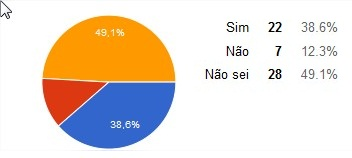
\includegraphics[scale=0.7]{figuras/questao6.jpg}
\caption{Gr�fico relacionado a quest�o 1 do question�rio de Governan�a de TI }
\label{figura13}  
\end{figure}
A Figura ~\ref{figura13} ilustra resumidamente a opini�o da cominidade
acad�mica em rela��o aos recursos de TI existentes na UFSM.

Na sequencia a quest�o.\textit{'' Em sua opini�o, as tr�s principais
necessidades de TI da UFSM campus  Frederico Westphalen s�o:''} entre outras
respostas os entrevistados disseram.
Melhora da internet - Capacita��o sobre o SIE - Cria��o de planilhas/sistemas para 
facilitar o acompanhamento e a avalia��o dos servi�os prestados e da popula��o atendida,
 melhoria na telefonia entre outras respostas.

Na Ultima quest�o: \textit{''De uma forma geral, o grau de satisfa��o que tenho
em rela��o a UFSM campus  Frederico Westphalen com os recursos de TI disponibilizados � condizente  
com minhas necessidades.''} Obteve 59 respostas onde 1 pessoas responderam
concordar totalmente com a quest�o (1,7\%), 36 concordaram (61\%), 6 manifestaram se
indiferentes (10,2\%), 14 discordaram (23,7\%) e 2 discordam totalmente (3,4\%).
 
 \begin{figure}[H]
\centering
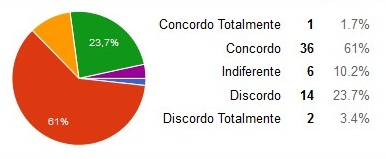
\includegraphics[scale=0.7]{figuras/questao8.jpg}
\caption{Gr�fico relacionado a quest�o 1 do question�rio de Governan�a de TI }
\label{figura14}  
\end{figure}
A Figura ~\ref{figura14} mostra resumidamente o resultado d quest�o a cima
citada mostrando no gr�fico de uma forma mais did�tica o resultado d satisfa��o
da comunidade acad�mica em rela��o aos recursos de Ti dispon�veis.

  \section{Trabalhos Relacionados}
\label{sec:trabalhosRelacionados}


  Mancini \cite{Mancini} desenvolveu um estudo de caso em uma 
  institui��o financeira de m�dio porte, descrevendo o processo de implanta��o 
  da GTI, abordando uma pesquisa qualitativa, com analise de documentos e da 
  observa��o participante. A organiza��o financeira utilizou um modelo de boas 
  pr�ticas de Governan�a Corporativa publicado pelo IBGC (Instituto Brasileiro de 
  Governan�a Corporativa). A organiza��o era dividida em tr�s �reas: Desenvolvimento 
  de Sistemas, Suporte T�cnico e Processos, com diversos problemas na �rea de TI, como: 
  imagem da TI ruim, desempenho da TI abaixo do esperado, projetos com altos custos e 
  baixo retorno de investimento, gerenciamento de projetos ineficaz e n�o alinhamento 
  das estrat�gias de neg�cios com as estrat�gias de TI. Devido a isso foi contratado 
  uma consultoria especializada para avaliar a organiza��o e seu n�vel de maturidade, 
  onde detectou-se que estava situada no n�vel 2 (Repetitivo) e o objetivo era atingir 
  o n�vel 3 (Definido), para isso foi elaborado o Planejamento do Projeto da governan�a 
  de TI para simplificar processos de TI, sendo monitorado, mensurados, e detectado os 
  desvios. O trabalho foi dividido em tr�s etapas, a primeira de alto risco, tudo 
  era realizado parcialmente sem muito controle. Na segunda, apesar de existirem 
  problemas, iniciava um maior uso da metodologia proposta, os processos de TI 
  estavam sendo usados parcialmente. Na terceira a organiza��o percebe os resultados 
  ao se atingir o n�vel 3- Definido que era o almejado, do framework COBIT, a partir 
  de ent�o se observou mudan�as na cultura da organiza��o, aderindo processos do COBIT. 
  Foi examinada a implanta��o de GTI por um per�odo de tr�s anos. Mesmo seguindo a 
  metodologia o estudo de caso apresenta limita��es, pois a incapacidade de 
  generaliza��o cientifica, por�m em outras organiza��es podem ocorrer de forma 
  diferente. No entanto diferindo do estudo realizado na UFSM uma institui��o de 
  ensino p�blica que foi estudado ferramentas j� existentes na universidade usando 
  como norteador o framework ITIL para analise de tal ferramenta, o estudo relacionado 
  implantou a Governan�a de TI em um institui��o financeira que basicamente busca o 
  lucro, usando frameworks e boas pr�ticas de Governan�a Corporativa publicado pelo 
  IBGC.
 
 
	
  Neves \cite{Neves} realizou um estudo de caso num empresa p�blica, criada para 
  gerir outras empresas federais, onde s�o oferecidos servi�os como consultorias, 
  desenvolvimento, acesso, suporte, provimento, treinamento e administra��o entre. 
  Na coleta de dados usou-se entrevistas, an�lise de relat�rios e planilhas, comparando
  os dados obtidos com o framework de boas pr�ticas do ITIL, desta forma o estudo tem 
  caracter�sticas explorat�rias, a pesquisa foi realizada em tr�s fases, coleta de 
  dados, an�lise e resultados, aplicadas no corpo t�cnico, identificando problemas do 
  dia-a-dia, analisando relat�rios de quantidade de atendimento mensal verificando onde 
  houve maior incid�ncias de chamadas. Finalizando realizando-se uma an�lise e amostra 
  aos t�cnicos dos cinco problemas mais frequentes, buscando solu��o. Ap�s foi feito 
  um diagnostico com identifica��o dos problemas tanto na parte operacional com na parte 
  dos lideres de equipes, identificando informa��es de falhas existentes e as solu��es 
  poss�veis, levantando dados num�ricos para quantificar informa��es. Depois de 
  identificados o problema foi feita uma segunda leitura dos mesmos, relacionando os 
  cinco mais frequentes e transcrevendo as de forma � facilitar a quantifica��o de 
  informa��es, dessa forma identificaram-se defici�ncias nos processos de diagn�sticos 
  e resolu��o de problemas, realizando um comparativo entre os resultados encontrados e 
  o framework de boas pr�ticas de ITIL. O gerenciamento de Problemas, tendo como escopo 
  a parte de diagn�stico e resolu��o de problemas, que no ITIL � contemplada dentro do 
  controle de problemas. Uma importante diferen�a � que o estudo de caso em quest�o foi 
  desenvolvido em uma institui��o de ensino enquanto que o estudo relacionado foi feito 
  em uma empresa que tem como fun��o gerir outras empresas p�blicas enquanto que o 
  estudo relacionado analisou o gerenciamento de problemas o estudo em quest�o na 
  UFSM procurou levantar portf�lios de servi�os e analisar os mesmos para assim fazer 
  um melhor uso de ferramentas j� existentes.
 
Morais \cite{Morais} realizou um estudo de caso usando uma abordagem qualitativa, 
interagindo apenas com os principais gestores de TI, essa pesquisa foi de natureza 
explorat�ria, primeiramente foi realizada uma pesquisa bibliogr�fica para levantamento 
de informa��es sobre a aplica��o de Governan�a de TI, Governan�a Corporativa e seus 
principais frameworks, em seguida uma elabora��o de um dossi� sobre a organiza��o. 
Realizando uma pesquisa de campo para identifica��o de problemas, coletando
informa��es com os gerentes da organiza��o, relacionando estas informa��es com os 
frameworks de boas pr�ticas identificando benef�cios e dificuldades, em seguida 
determinado a��es a serem tomadas. Objetivando dessa forma, alinhar a estrat�gia 
de TI com a estrat�gia da organiza��o, realizando um plano de a��o designando gestores 
para a realiza��o dentro da organiza��o, este projeto foi realizado em 18 meses.
Ap�s analise de dados obtidos, foi constru�do o mapa estrat�gico de TI, identificando 
melhores pratica para cada �rea da organiza��o, visando a melhoria na cultura da 
organiza��o. Para a realiza��o de tais trabalhos o COBIT foi um instrumento viabilizador 
orientando as a��es para desenvolver instrumentos de avalia��o b�sica. Tamb�m o ITIL foi 
usado na orienta��o de pr�ticas na organiza��o, para aprimorar a gest�o de servi�os. 
O PMBOK tamb�m fez parte do processo de melhoria dando apoio aos lideres do neg�cio, 
aliando assim para atingir objetivos pr�-estabelecidos, resultando no alinhamento de TI 
aos neg�cios da organiza��o, COBIT foi um dos principais norteadores, enquanto que para 
o estudo de caso na UFSM, o framework ITIL foi o fundamentador da pesquisa disponibilizando 
suporte para analise e descri��o de dados levantados, identificando portf�lio de servi�os.
         
 Masson~\cite{Masson} realizado uma pesquisa na Administra��o P�blica, o objetivo desta 
 pesquisa foi avaliar, junto a �rg�os da Administra��o P�blica Federal, o alinhamento da 
 Governan�a de TI com a Governan�a Corporativa. Esta investiga��o utiliza a abordagem 
 quantitativa. Os dados referentes � Governan�a Corporativa e � de TI e os principais 
 modelos de governan�a foram obtidos em pesquisa documental. Foram aplicados os instrumentos 
 de coleta de dados: pesquisa em bases de dados, documentos organizacionais e question�rios
 semifechados. A pesquisa foi respondida por respons�veis da �rea de TI, ap�s analise foi 
 conclu�do que a Governan�a de TI era pouco ou nada usado como auxilio na tomada de decis�o. 
 Os resultados obtidos na pesquisa, remetem a uma baixa atua��o da Alta Administra��o na 
 Governan�a de TI nas institui��es pesquisadas. O estudo relacionado anteriormente difere-se 
 do realizado na UFSM campus de Frederico Westphalen, por este ter usado como
 framework boas pr�ticas do ITIL e do ISO/IEC38500 como norteadores para analisar e 
 alinhar TI a ferramenta Help Desk da organiza��o. Enquanto que Masson em seu estudo busca o 
 alinhamento de Governan�a de TI a Governan�a Corporativa.


	   

  %\begin{}
%Aqui vai o conclusao\ldots
%\end{conclusoes}
\section{Conclus�es}
\label{sec:conclusoes}
Ap�s estudo realizado foi poss�vel concluir que Governan�a de TI � uma ferramenta 
muito importantes para que organiza��es consigam manter se em pleno funcionamento, 
para isso existem frameworks para auxiliar nessa estrutura��o entre eles os mais usados 
s�o o COBIT, ITIL e ISO/IEC38500, o embasamento te�rico direcionou o estudo e dessa forma 
fez-se compreender que Governan�a de TI esta em pleno desenvolvimento e sua import�ncia � 
cada vez mais vis�vel. Quando observado a utiliza��o de Governan�a de TI na Universidade 
Federal de Santa Maria no campus de Frederico Westphalen viu-se que e muito pouco utilizada.

Com o avan�o da tecnologia e a acelera��o cada vez maior da mesma �  importante o 
acompanhamento de Governan�a de TI em qualquer organiza��o seja ela p�blica ou privada 
de qualquer tamanho, pois d�o suporte a tomada de decis�es, o mais importante � que tudo 
que existir de controle na institui��o pode ser aproveitado n�o � necess�rio que seja 
come�ado do zero para existir Governan�a de TI as ferramentas existentes,
 para dai em diante ser incrementado novos planos de implementa��o, as
 organiza��es precisam ser controladas e para tr controle elas precisam ser
 gerenciadas, por essa resalva que que governan�a e gerencia devem caminhar
 juntas para dessa forma atingir os objetivos desej�veis.
 
Por�m ao estudar Governan�a de TI � encontrada diversas dificuldades entre elas est�o a 
necessidade de investimentos tanto em recursos financeiros quanto em recursos humanos, 
dificultando dessa forma a implanta��o de Governan�a de TI, pois, h� a
necessidade de pessoas treinadas e com tempo dedicado nesse processo, para dessa
forma alinha-la a ao neg�cio. Uma alternativa relevante na quest�o � o uso de
ferramentas livres dispon�veis no software p�blica, neste trabalho voi estudado
a ferramenta CITSMART, est� por sua vez possibilita a cobertura de todas as
�reas da UFSM campus de FW, sendo que a mesma disponibiliza de servi�os bem
completos, por�m a maior entrave ficaria no treinamento de pessoa, sendo que a
mesma por ser ampla demandaria de m�o de obra treinada.

Por Governan�a de TI ser um assunto t�o em alta na atualidade e ser um assunto que cada 
vez mais discutido pelas organiza��es � poss�vel desenvolver estudos, com esse
intuito foi realizado estudo na UFSM  campus de FW analisando a ferramenta Help
Desk do campus verificando que a mesma n�o � institucionalizada, � usada apenas para 
controle interno do setor, foi feito um levantamento de portf�lio de servi�os da mesma 
onde visto que a ferramenta suporta no apenas um servi�o que � a abertura de chamados onde s�o cadastradas as atividades 
realizadas e posteriormente gerados relat�rios. Para poder ser feita est� pesquisa 
anteriormente foi realizado uma pesquisa liter�ria de Governan�a de TI e seus principais 
frameworks, COBIT, ITIL e ISO/IEC38500 para dessa forma embasar a pesquisa e definir assim 
portf�lio a ser seguido, optando por utilizar ITIL e ISO para suportar a pesquisa. 

Governan�a � um assunto muito amplo dessa forma como uma das ferramentas de
estudo foi aplicado um question�rio no campus de FW para dessa form oobter
informa��es onde foi poss�vel observam a amplitude de alcance que a TI tem, por
esse motivo � poosivel afirmar que � necess�rio um maior controle da mesma
alinhando ela a todas as �reas da organiza��o.

Ap�s o estudo da ferramenta Help Desk utilizada na UFSM campus de FW, o
question�rio aplicado com a comunidade acad�mica e a ferramenta CITSMART, �
poss�vel tra�ar os passos futuros, a an�lise de novas ferramentas possibilita
aumentar o conhecimento e assim ter uma perspectiva de quanto Governan�a de TI �
importante em uma organiza��o. A coleta de novos dados e a institucionaliza��o
da ferramenta Help Desk, que at� momento � utilizada somente para controle
interno do setor de TI da universidade, poderia ser um come�o pra o alinhamento de TI
com as demais �reas da universidade.

 
 
 %%%-----------------------------------%% END ARTIGO
 
%%% Referencias bibliograficas no padrao da SBC
\bibliographystyle{sbc}

%%% Referencias bibliograficas no padrao da IEEE
%\bibliographystyle{IEEEtran} 
 
 %%% Nome do arquivo .bib contendo as suas referencias bibliograficas
\bibliography{referencias}

 
\end{document}
